\documentclass[aspectratio=169]{beamer} %% for 16:9 use this line
%%\documentclass{beamer} %% For 4:3 ratio use this line
\usepackage[utf8]{inputenc}
\usepackage[T1]{fontenc}
\usepackage{lipsum} 
\usepackage{bm}
\usepackage{graphicx}
\usepackage{animate}
\usepackage{amsmath}
\usepackage{subcaption}
\usepackage{tikz}
\usepackage{soul}
\usepackage[most]{tcolorbox}
\usepackage{amssymb}% http://ctan.org/pkg/amssymb
\usepackage{pifont}% http://ctan.org/pkg/pifont
\newcommand{\cmark}{\ding{51}}%
\newcommand{\xmark}{\ding{55}}%
\captionsetup[figure]{font=footnotesize}
% import citation package
\usepackage[backend=biber, style=authoryear]{biblatex}
\addbibresource{../../conference/biblio.bib}
\AtBeginBibliography{\small}
\DeclareMathOperator*{\argmin}{\arg\!\min}
% footnote without number
\newcommand\blfootnote[1]{
\begingroup
\renewcommand\thefootnote{}\footnote{#1}
\addtocounter{footnote}{-1}
\endgroup
}

\usetheme{CEA2023}
\setlength{\columnsep}{0.05cm}
\title[Café Thésard]
{Marius Duvillard - Construction du jumeau numérique du procédé de mélange/broyage des combustibles par assimilation de données} %optional
\subtitle{Café Thésard 28/06/2024}
\date[28-06-2024] %optional
{28 juin 2024}
\author[M. Duvillard] %optionam
{Marius Duvillard \inst{1} \inst{2} \texttt{(\small marius.duvillard\myat cea.fr)} \\
Olivier Le Maître \inst{2} \inst{3} \texttt{(\small olivier.le-maitre\myat polytechnique.edu)} \\
Michel Freyss \inst{1} \texttt{(\small michel.freyss \myat cea.fr)}\\
}

\institute[short-inst]{
 \inst{1} CEA DES/IRESNE/DEC/SESC Cadarache 
 \inst{2} Centre de Mathématiques Appliquées, Ecole Polytechnique 
 \inst{3} CNRS, Inria
}

% uncomment the following lines if you do not want dedicated outlines before
% each section
\AtBeginSection{}

% use your thanks-message in the last frame
\setvalue{\ThxMessage}{Thanks! Any questions?}
% Change the logo 
\titlegraphic{logos/LOGO_CEA_ORIGINAL.png}

% introduce another logo for a second author or affiliation
% secondlogo applies to the first page only
\setvalue{\secondlogo}{logos/Polytechnique_logo.pdf}

\begin{document}

% info: the plain removes the footline from the titlepage; noframenumbering
% neglects it from the total count of the slides
\begin{frame}[decorated] %Decorated bring the logo and corner
    \titlepage
\end{frame}

\begin{frame}[righttransition]{Outline} % or Table of Contents
    \tableofcontents
\end{frame}

\section{Introduction}
\subsection{Contexte industriel et scientifique}
%1
\begin{frame}{Problématique Industrielle}
    \vspace{-0.25cm}
    \begin{columns}[t]
        \begin{column}{0.5\textwidth}
            \small
            \begin{block}{Fabrication du combustible MOX}
                Combustible nucléaire à base de $PuO_2$ + $UO_2$
                \begin{figure}
                    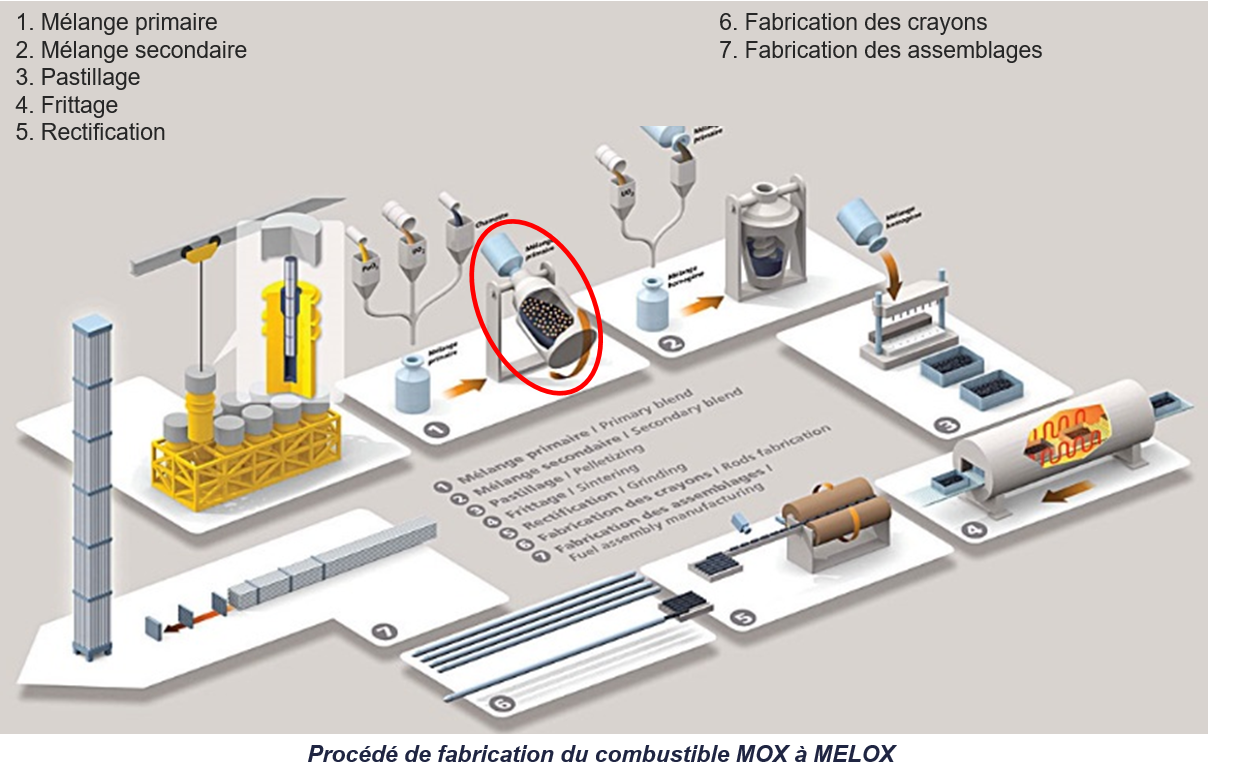
\includegraphics[width=\textwidth]{../CSI_2024/image/cycle_combustible.png}
                    % \caption*{procédé MiMas mis en œuvre à l’usine MELOX pour la préparation du combustible MOX [Orano, 2017]}
                \end{figure}
                Etude de l'étape de mélange et de broyage des poudres
            \end{block}
        \end{column}
        \begin{column}{0.5\textwidth}
            \small
            \begin{figure}
                \centering
                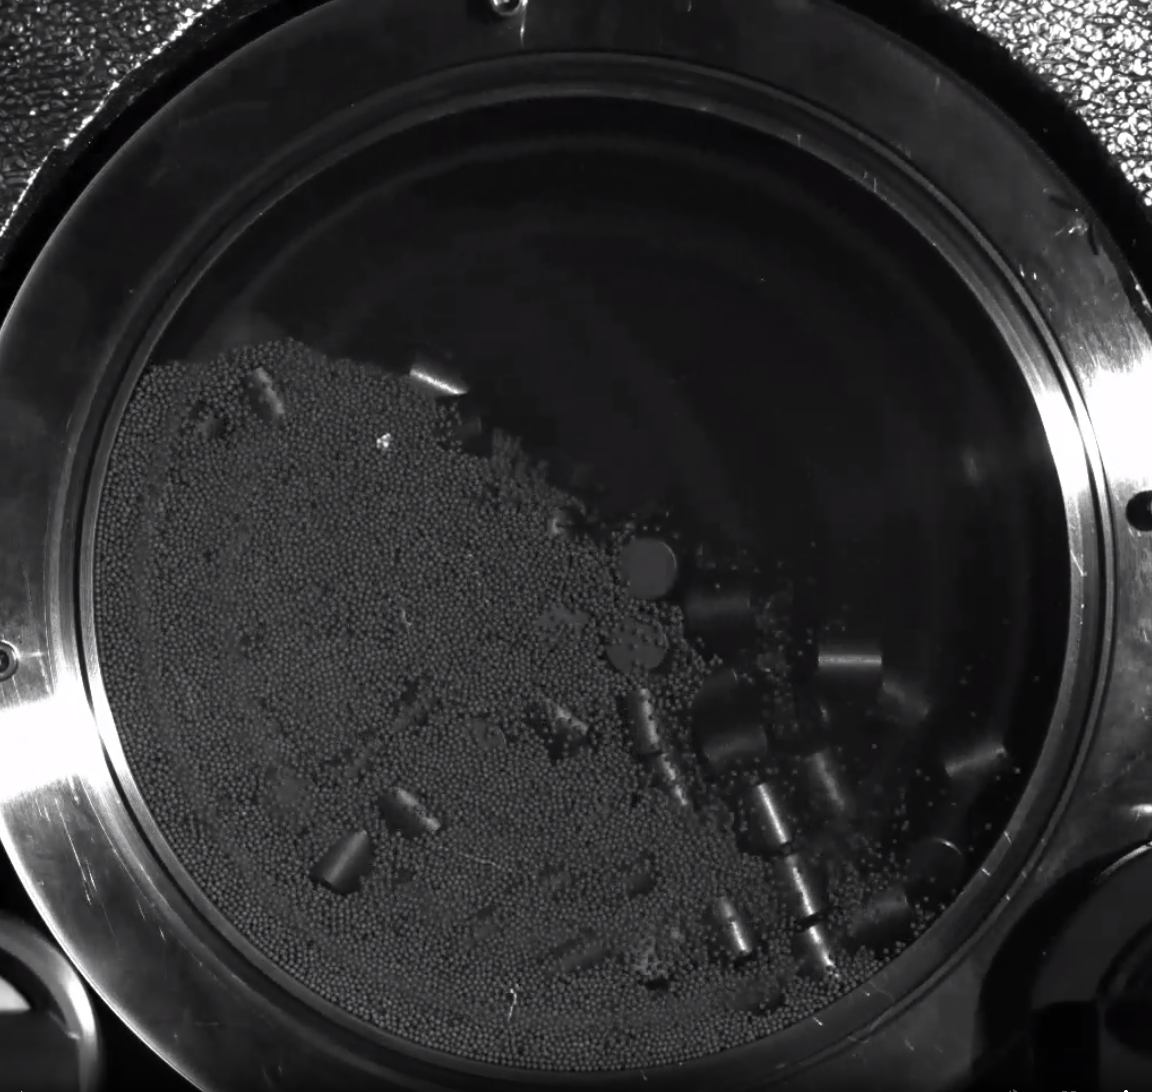
\includegraphics[width=0.5\textwidth]{../CSI_2024/image/broyage.png}
            \end{figure}
            \textbf{Objectifs :}
            \begin{itemize}
                \item Améliorer l'homogénéité des poudres $UO_2 + PuO_2$
                \item Réduire la taille des grains
            \end{itemize}
            Mécanismes de \textbf{mélange} et de \textbf{fragmentation} complexes
        \end{column}
    \end{columns}
\end{frame}

%2
\begin{frame}{Bro-IA-ge: Jumeau numérique du mélangeur broyeur}
    \begin{itemize}
        \item \textbf{Définition} [Digital twin consortium] : “A digital twin is a virtual representation of real-world entities and processes, synchronized at a specified frequency and fidelity.”
        \item \textbf{Multidisciplinaire} : Modélisation physique, résolution de problème inverse, quantification d’incertitude, IA,\dots
    \end{itemize}
    \vspace{-0.5cm}
    \begin{columns}[t]
        \begin{column}{0.45\textwidth}
            \begin{figure}
                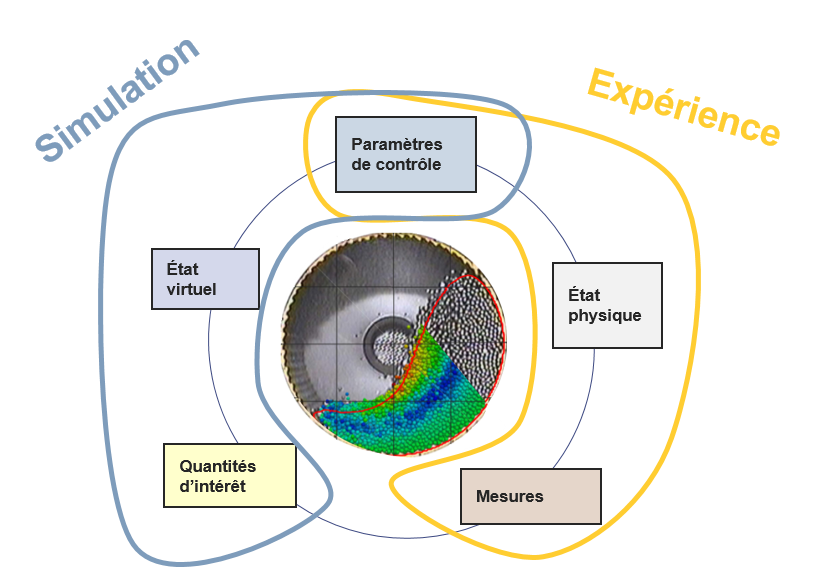
\includegraphics[width=1.1\textwidth]{./images/Jumeau_numerique.png}
            \end{figure}
        \end{column}
        \begin{column}{0.55\textwidth}
            \begin{block}{Objectifs}
                \begin{itemize}
                    \item \textbf{Compréhension/Optimisation/Surveillance}
                    \item \textbf{Modélisation}
                          \begin{tcolorbox}[colframe=red, colback=white, boxrule=0.5mm, arc=0mm, outer arc=0mm]
                              \item \textbf{Assimilation de données} mise à jour de l’état en fonction des données de capteurs
                              \item \textbf{Filtrage / Prédiction} estimation de l’état actuel ou futur
                          \end{tcolorbox}
                    \item \textbf{Apprentissage}
                          Réduction du temps de calcul, maintenance prédictive, contrôle commande...
                \end{itemize}
            \end{block}
        \end{column}
    \end{columns}
\end{frame}

%4 Simulation
\begin{frame}{Simulation du broyeur à boulets - Méthodes particulaires}
    \vspace{-0.25cm}
    \begin{columns}[t]
        \begin{column}{0.5\textwidth}
            \textbf{Discret Element Method} \\
            \begin{figure}[b]
                \animategraphics[loop, autoplay, width=0.5\textwidth]{10}{../CSI_2024/image/rot_drum_dem/rot_drum_dem-}{0}{199}
            \end{figure}
            \begin{itemize}
                \item Méthode N-Body
                \item Interaction basées sur le contact frottant
                \item Modélisation à l'échelle des particules
                \item Implémentation des phénomènes physique: Fragmentation, agglomération
            \end{itemize}
            \vfill

            % \begin{itemize}
            %     \item Positions ne peuvent être modifié directement
            % \end{itemize}
        \end{column}

        \begin{column}{0.5\textwidth}
            \textbf{Material Point Method} \\
            \begin{figure}[b]
                \animategraphics[loop, autoplay, width=0.6\textwidth]{10}{../../conference/images/rot_drum_mix/rot_drum_mix-}{0}{149}
            \end{figure}
            \begin{itemize}
                \item Méthode sans maillage
                \item Discrétisation d'une solution continue à l'aide d'une discrétisation particulaire
            \end{itemize}
            \vfill

        \end{column}
    \end{columns}
\end{frame}

\subsection{Assimilation de données}
%5
\begin{frame}{Assimilation de données}
    \begin{figure}
        \centering
        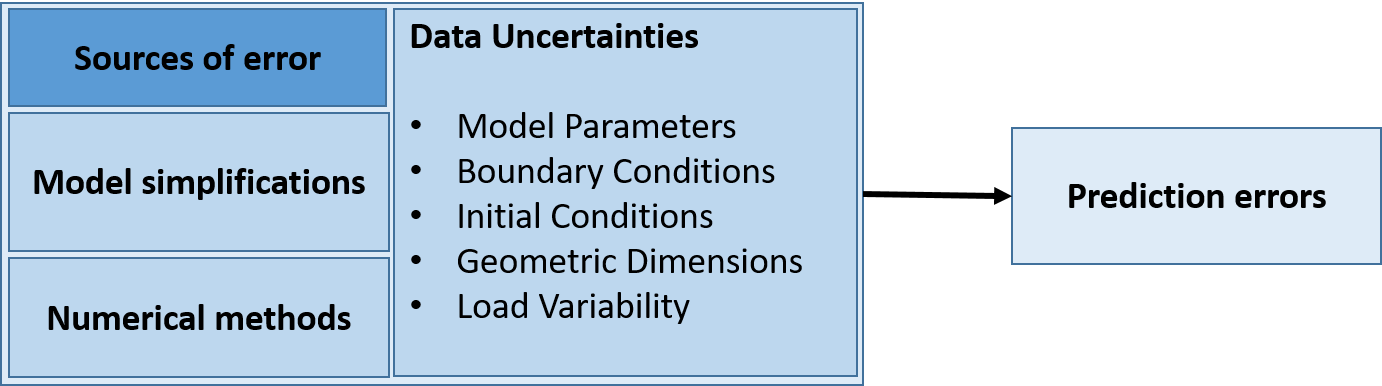
\includegraphics[width=0.7\textwidth]{../../conference/images/source_of_uncertainties.png}
    \end{figure}

    \textbf{Objectif :} Incorporer des observations pour réduire l'erreur de prédiction et les incertitudes
    \begin{figure}
        \centering
        \alt<2>{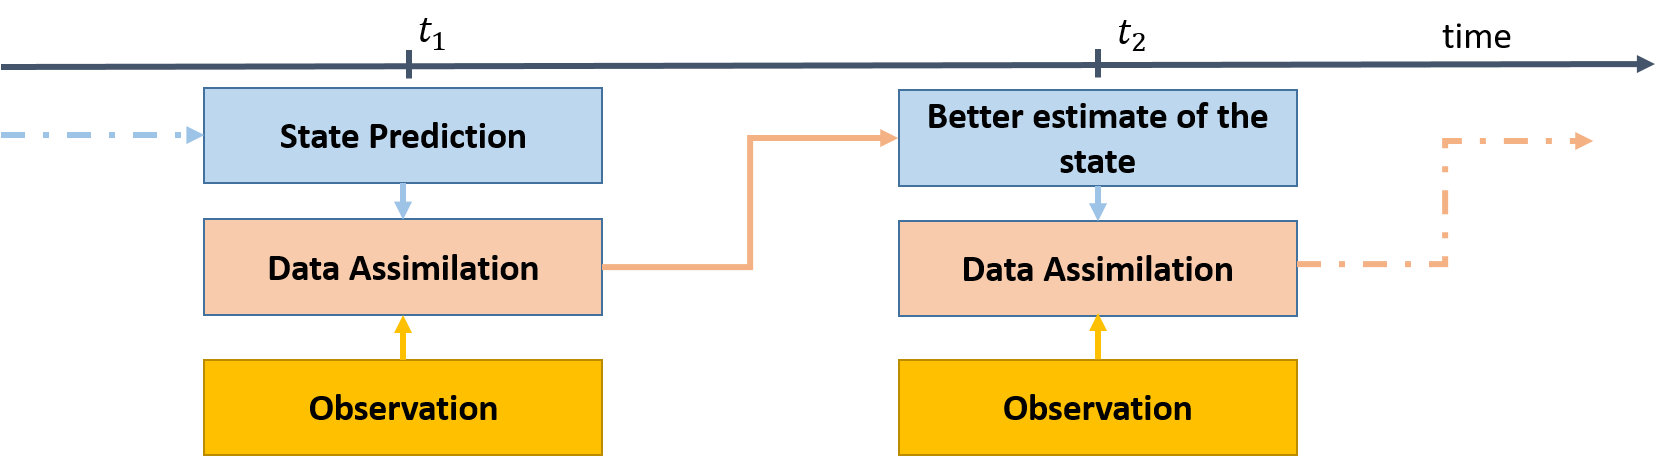
\includegraphics[width=0.8\textwidth]{../../conference/images/da_scheme2.png}}{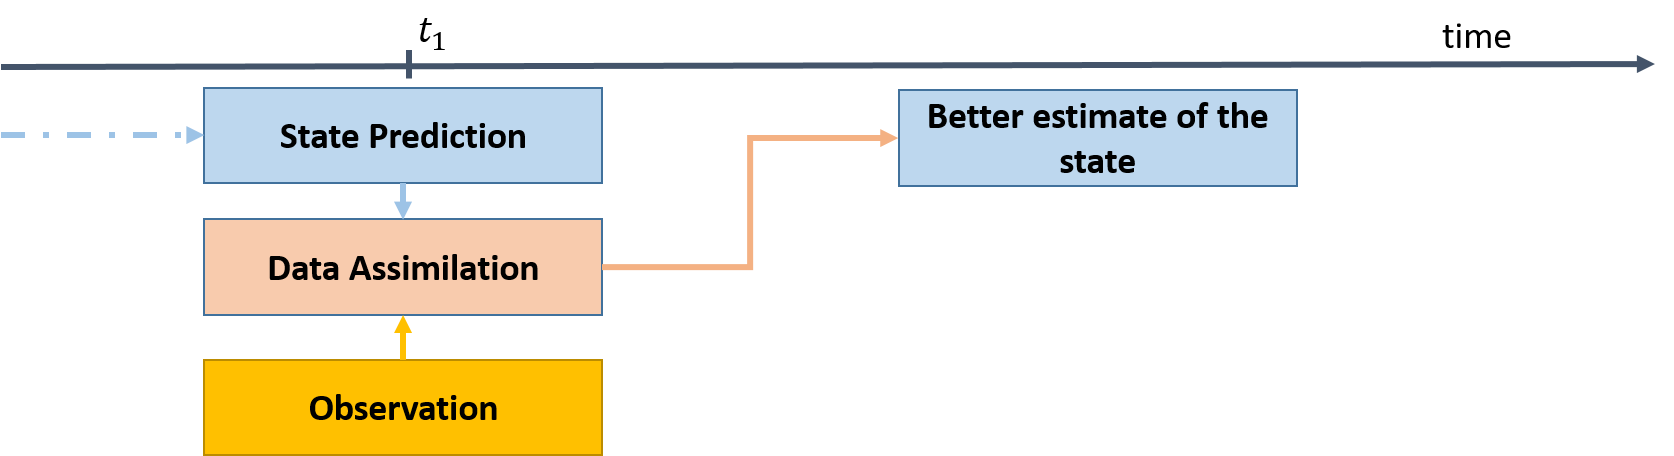
\includegraphics[width=0.8\textwidth]{../../conference/images/da_scheme1.png}}
    \end{figure}
    \vfill
\end{frame}

%3 Données
\begin{frame}{Données mesurées}
    \begin{figure}[t]
        \centering
        \begin{subfigure}[b]{0.3\textwidth}
            \only<1>{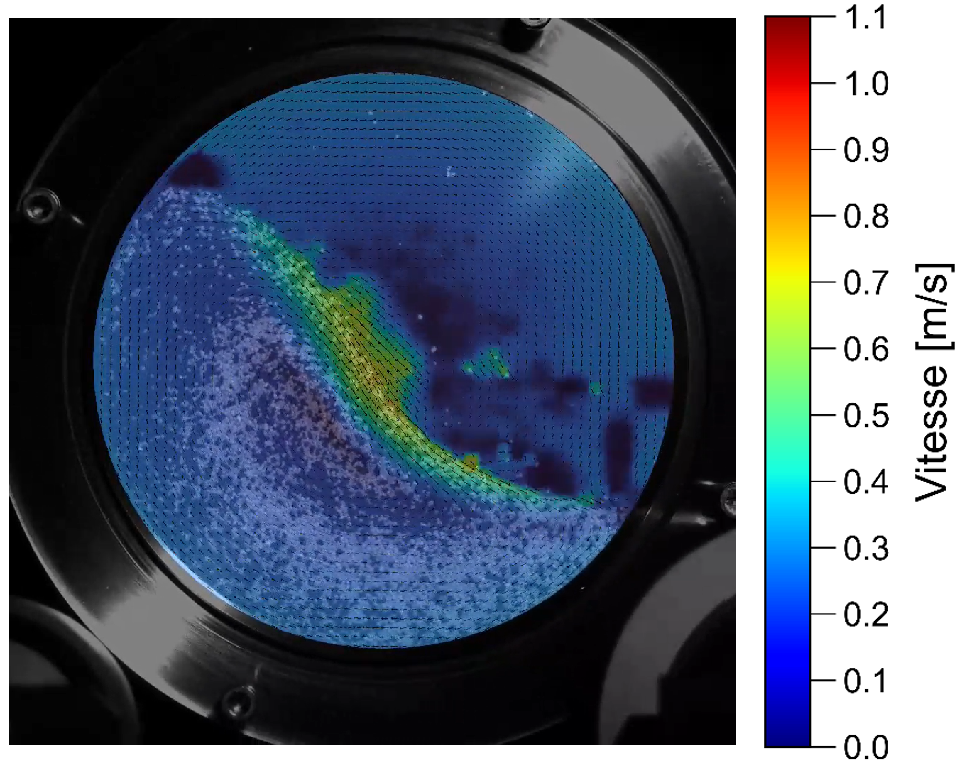
\includegraphics[width=\textwidth]{../CSI_2024/image/mesure_pic.png}
            }
            \only<2->{\begin{tcolorbox}[colframe=red, colback=white, boxrule=0.5mm, arc=0mm, outer arc=0mm, boxsep=0mm, left=0mm, right=0mm, top=0mm, bottom=0mm]
                    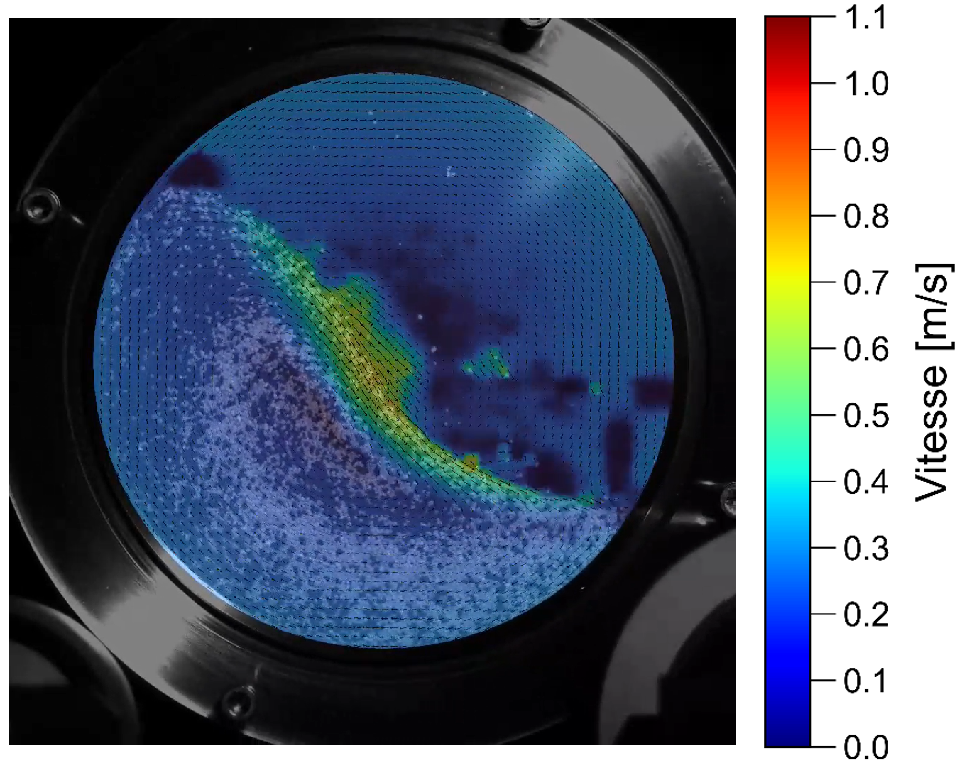
\includegraphics[width=\textwidth]{../CSI_2024/image/mesure_pic.png}
                \end{tcolorbox}}
            \caption*{particule Image Velocimetry}
        \end{subfigure}
        \hfill
        \begin{subfigure}[b]{0.3\textwidth}
            \only<1>{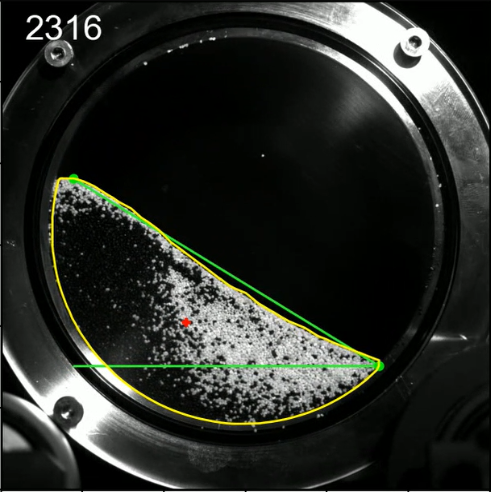
\includegraphics[width=\textwidth]{../CSI_2024/image/mesure_theta.png}}
            \only<2->{\begin{tcolorbox}[colframe=red, colback=white, boxrule=0.5mm, arc=0mm, outer arc=0mm, boxsep=0mm, left=0mm, right=0mm, top=0mm, bottom=0mm]
                    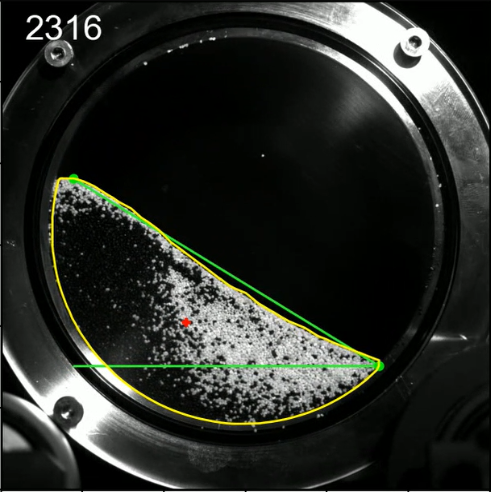
\includegraphics[width=\textwidth]{../CSI_2024/image/mesure_theta.png}
                \end{tcolorbox}}
            \caption*{angle de repos dynamique}

        \end{subfigure}
        \hfill
        \begin{subfigure}[b]{0.3\textwidth}
            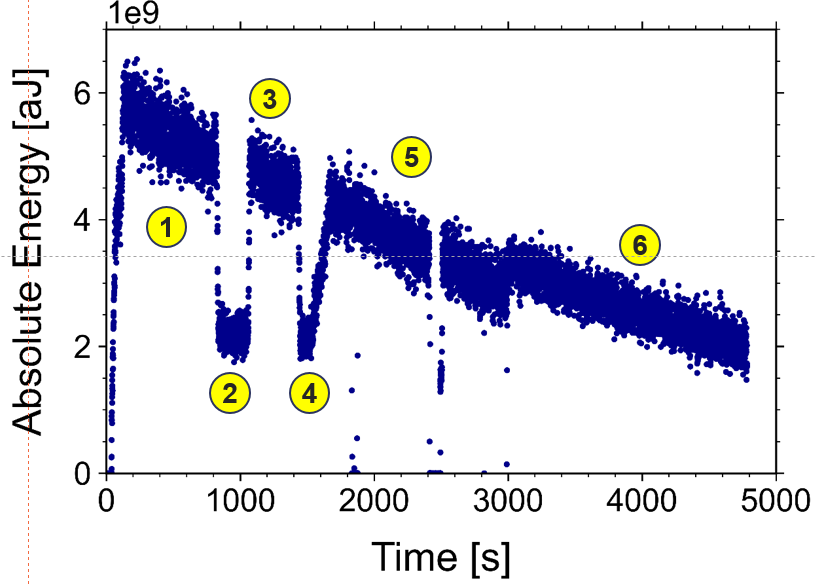
\includegraphics[width=\textwidth]{../CSI_2024/image/mesure_ea.png}
            \caption*{mesures electro-acoustique}
        \end{subfigure}
    \end{figure}
    \visible<2->{Les données doivent pouvoir être \textbf{confrontées} à la simulation (pouvoir être \textbf{prédites})}
\end{frame}
%6
\begin{frame}{Filtre de Kalman d'Ensemble (EnKF)}
    \begin{itemize}
        \item Extension du \textbf{Filtre de Kalman} avec un \textbf{ensemble} de membres pour estimer et propager l'incertitude de l'état~\cite{evensen_sequential_1994}
        \item Adapté à un espace d'état \textbf{non-linéaire} et \textbf{de haute dimension}
    \end{itemize}
    \vspace{-0.4cm}
    \begin{columns}[t]
        \begin{column}{0.65\textwidth}
            \small

            \textbf{Étapes de l'EnKF} (nous notons $u(\cdot, t_{k}) = u_k(\cdot)$) :
            \begin{itemize}
                \item \textbf{Initialisation} : \\
                      Échantillonner $N_{\text{ens}}$ champs $\textcolor{blue}{\left\{u_{i,0}\right\}_{i=1}^{N_{\text{ens}}}} \stackrel{iid}{\sim} U_0$
                \item \textbf{Propagation} : de $t$ à $t_{k+1}$ : \\
                      $\textcolor{blue}{ u^f_{i, k+1}} = \mathcal M(u_{i, k}), \quad i = 1, \dots, N_{\text{ens}}$
                \item \textbf{Mesure et prédiction} à $t_{k+1}$ : \\
                      mesurer $\textcolor{glycine}{y_{k+1}}$, \\
                      prédiction $\textcolor{glycine}{h^i_{k+1}} = \mathcal H (\textcolor{blue}{ u^f_{i, k+1}}) \quad i = 1, \dots, N_{\text{ens}}$
                \item \textbf{Analyse} : une combinaison linéaire pondérée de $u^f_{i,k+1}$ \\
                      $\textcolor{ceared}{u^a_{i, k+1}} = \textcolor{blue}{ u^f_{i, k+1}} + \sum_{j=1}^{N_{\text{ens}}} \textcolor{glycine}{\bm F_{ij}} \textcolor{blue}{ u^f_{j,k+1}}$, \\ où $\textcolor{glycine}{\bm F}$ dépend de $\left(\textcolor{glycine}{y_{k+1}, \left\{h_{i, k+1}\right\}_{i=1}^{N_{\text{ens}}}}\right)$\footnotemark[1]
            \end{itemize}
            \vspace{0.25cm}

        \end{column}
        \begin{column}{0.4\textwidth}

            \begin{figure}[t]
                \centering
                \only<1>{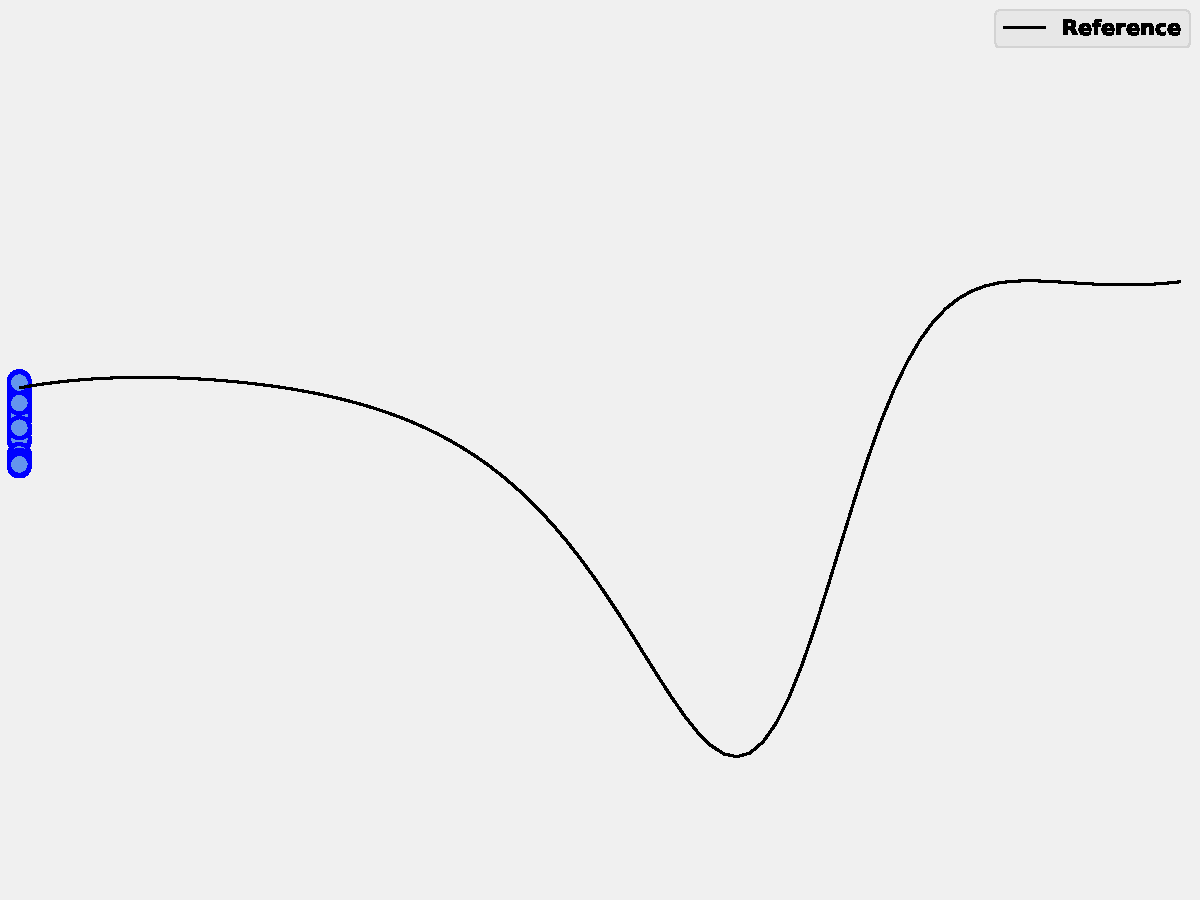
\includegraphics[width=\textwidth]{../../conference/images/enkf_traj/enkf_lorenz_init.pdf}}
                \only<2>{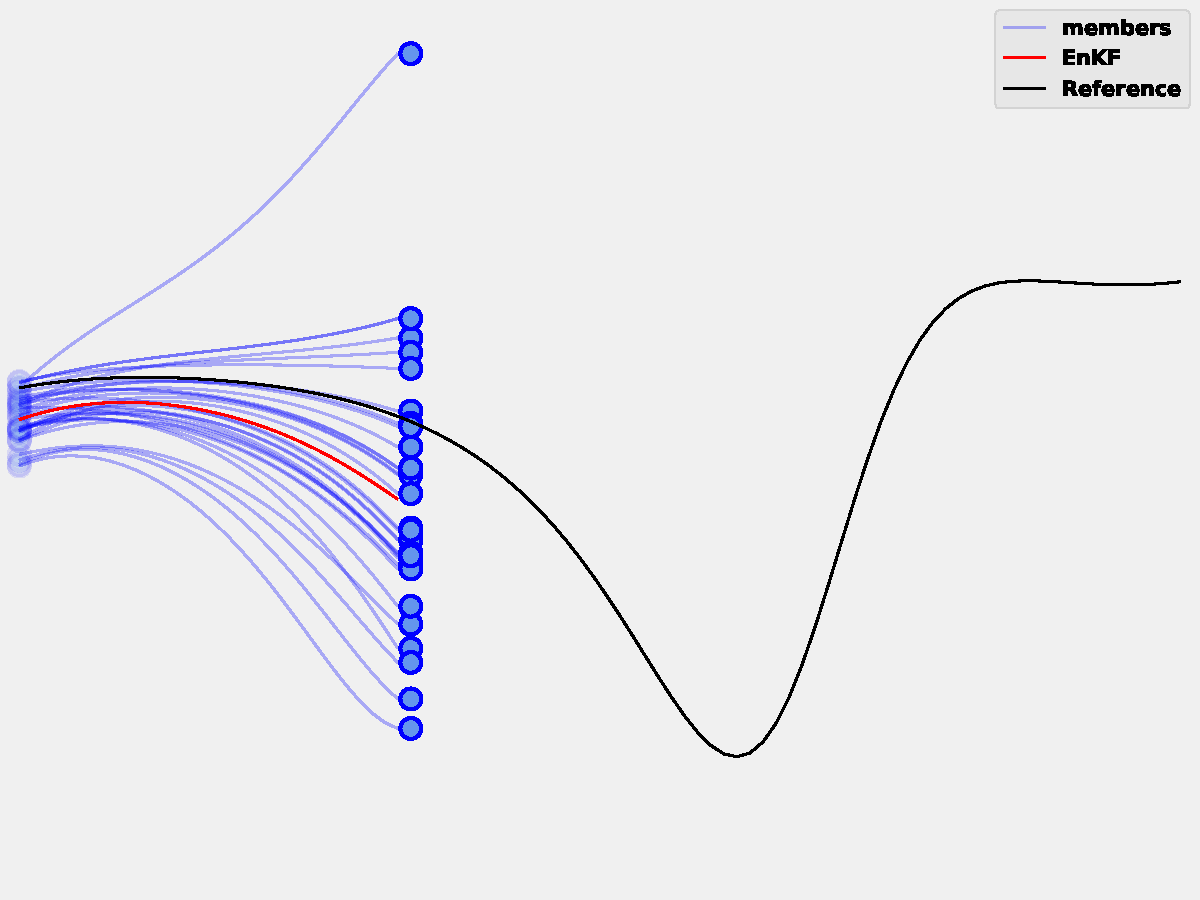
\includegraphics[width=\textwidth]{../../conference/images/enkf_traj/enkf_lorenz_prop.pdf}}
                \only<3>{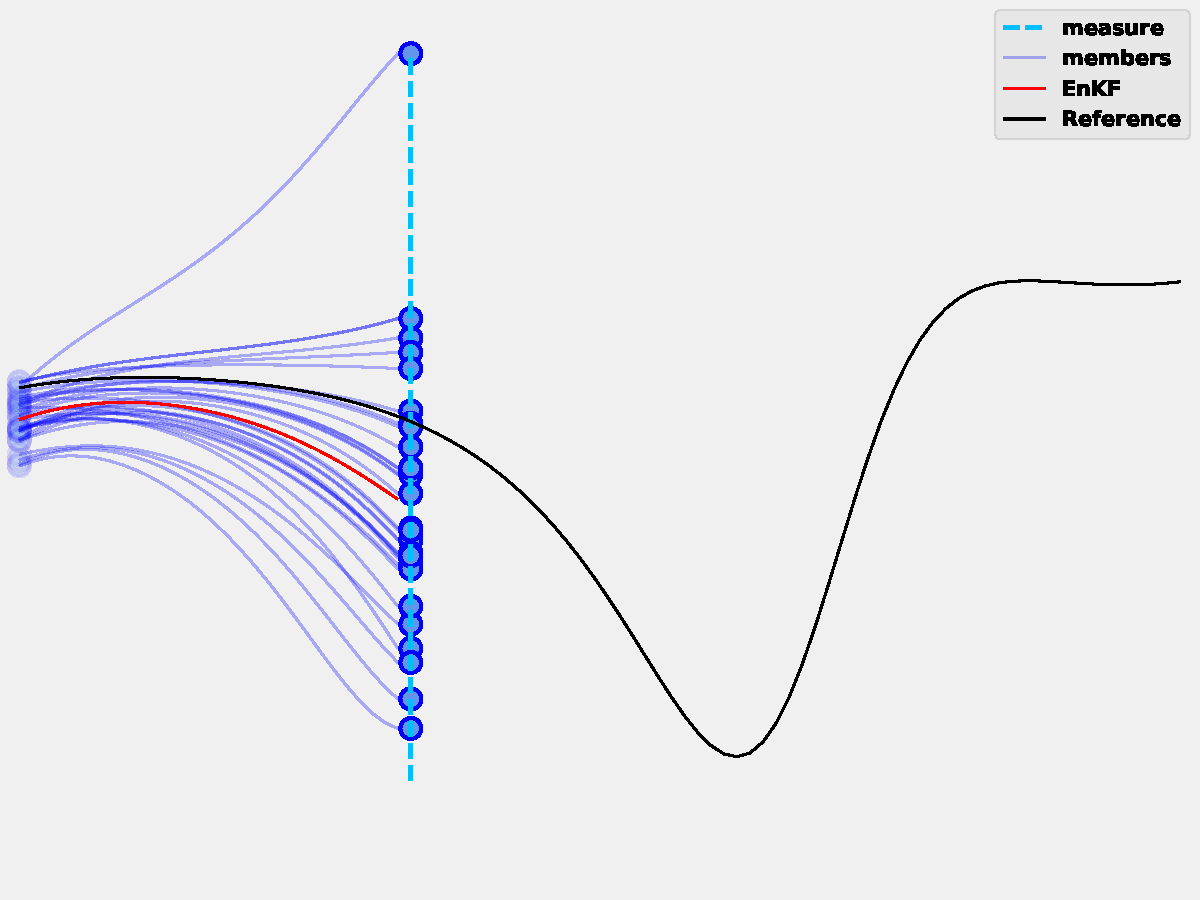
\includegraphics[width=\textwidth]{../../conference/images/enkf_traj/enkf_lorenz_measure.pdf}}
                \only<4>{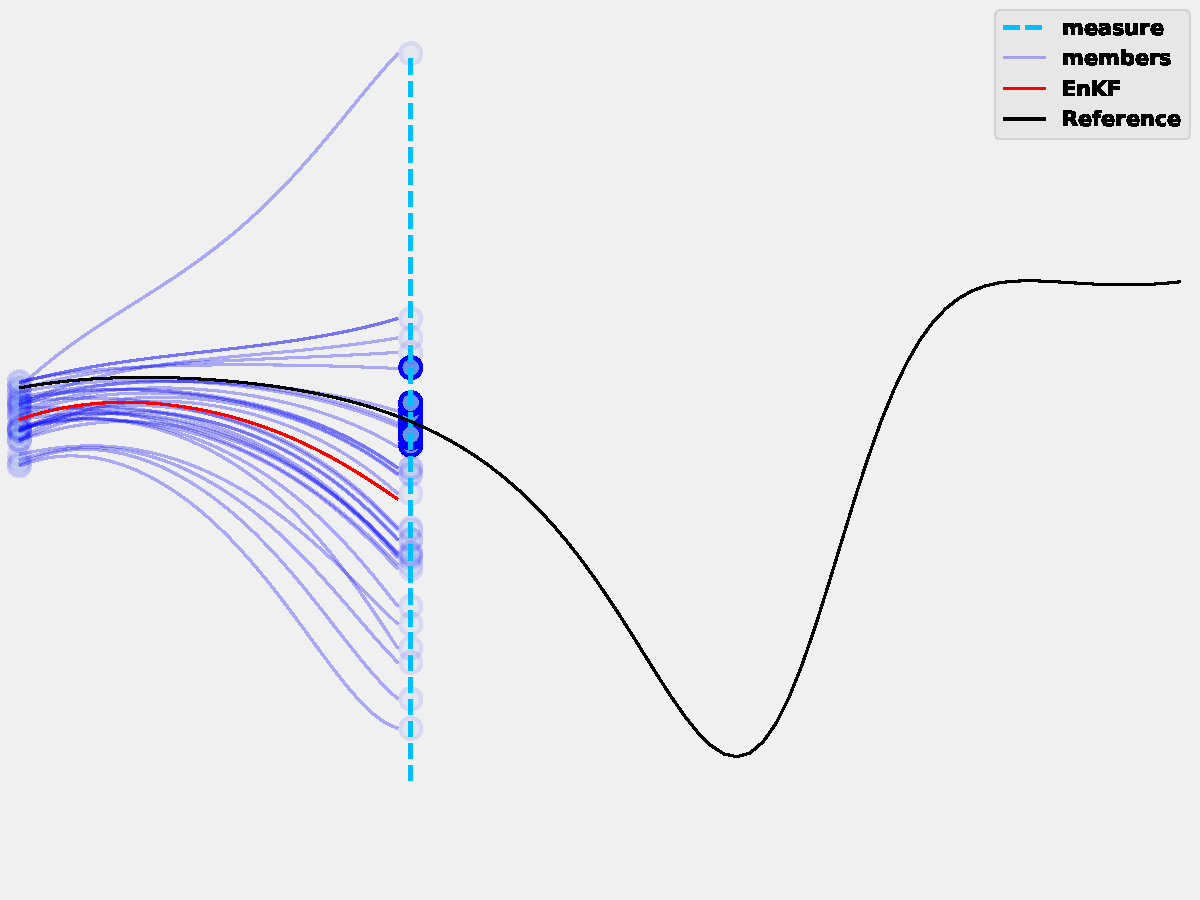
\includegraphics[width=\textwidth]{../../conference/images/enkf_traj/enkf_lorenz_assim.pdf}}
                \only<5>{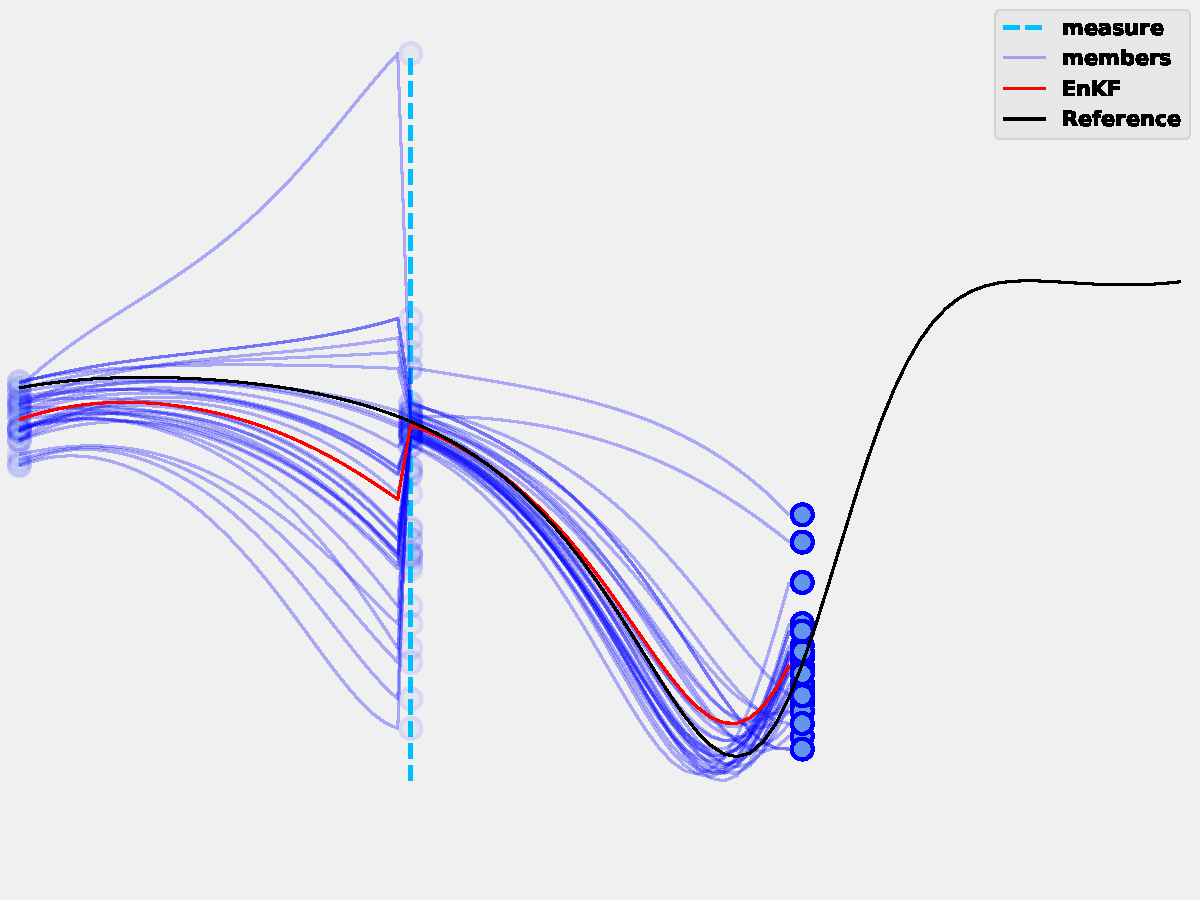
\includegraphics[width=\textwidth]{../../conference/images/enkf_traj/enkf_lorenz_prop2.pdf}}
                \only<6>{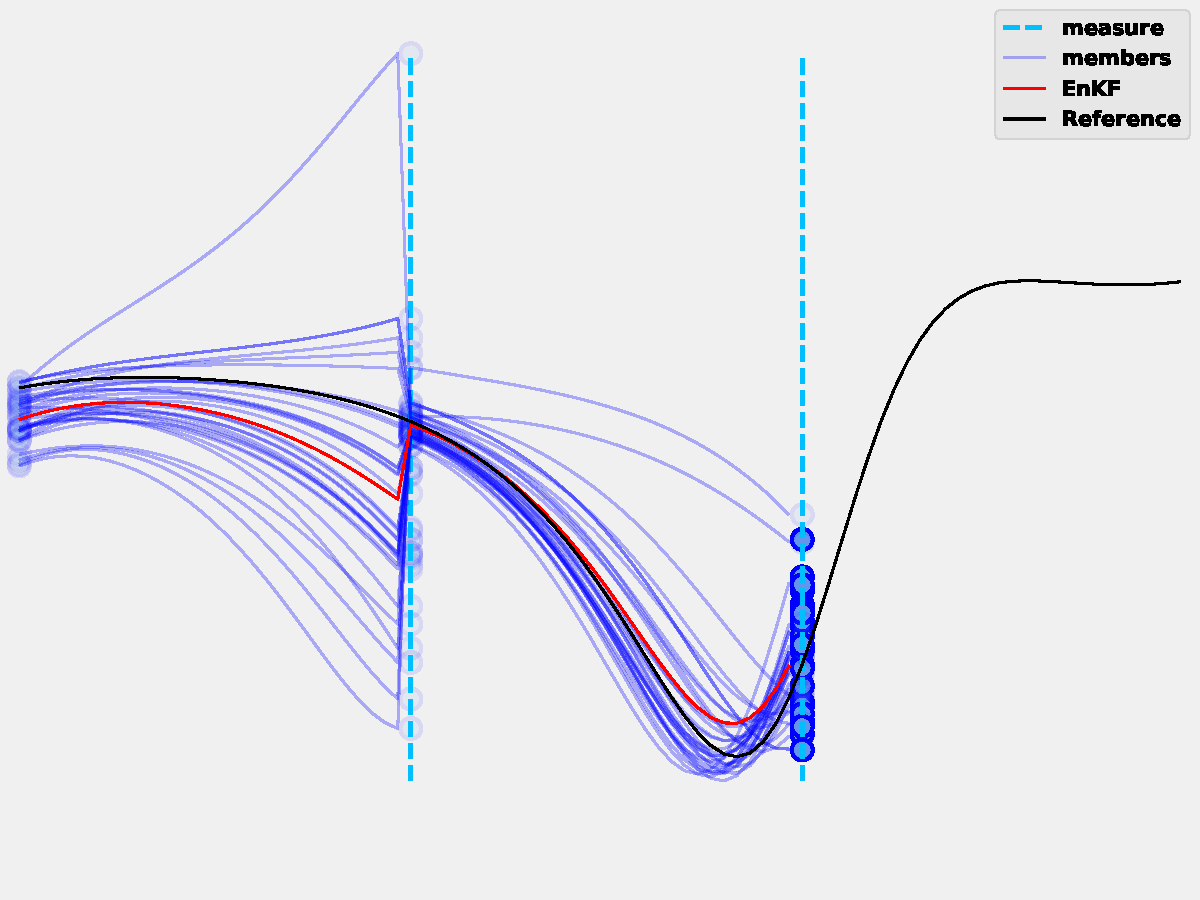
\includegraphics[width=\textwidth]{../../conference/images/enkf_traj/enkf_lorenz_assim2.pdf}}
                \only<7->{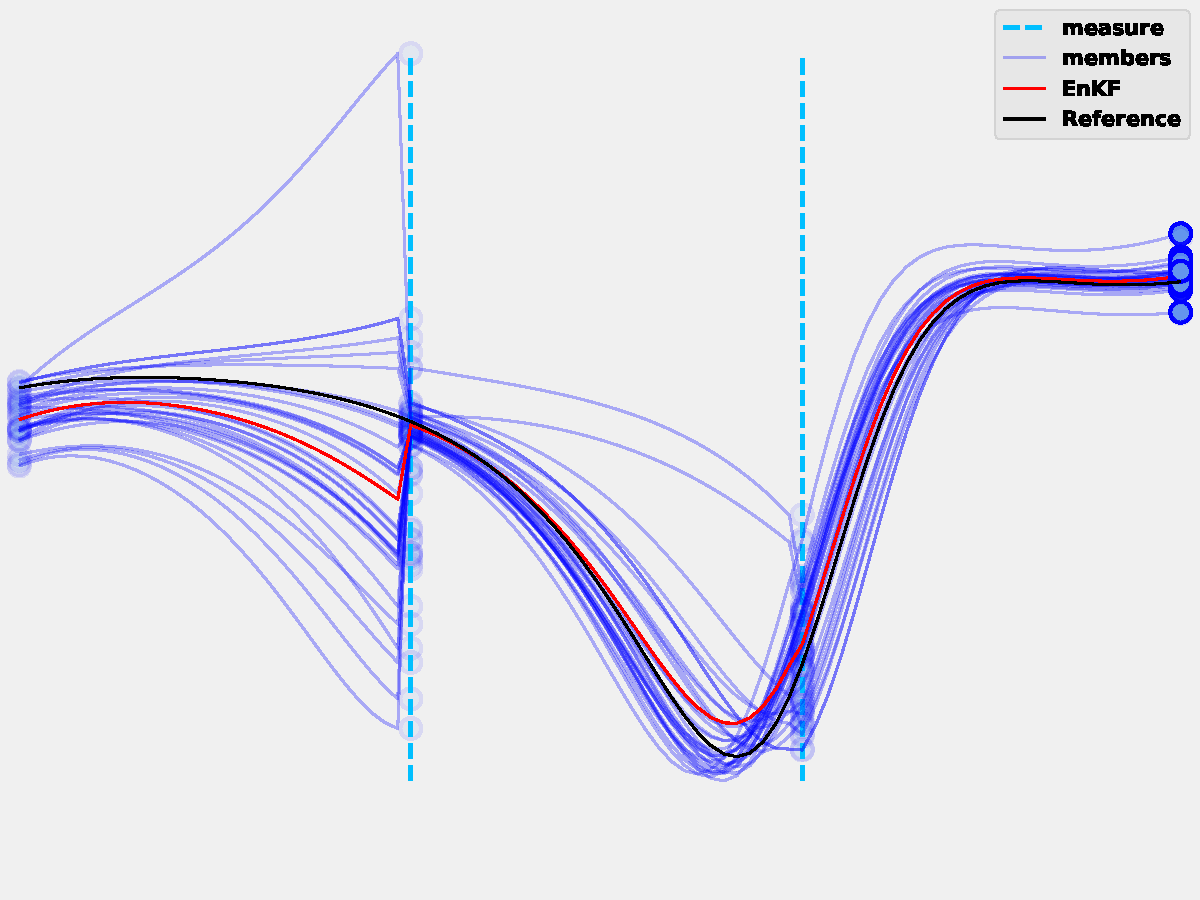
\includegraphics[width=\textwidth]{../../conference/images/enkf_traj/enkf_lorenz_final.pdf}}
            \end{figure}
            \visible<8->{\textcolor{ceared}{\small Comment appliquer cette correction aux simulations sans maillage ?}}
        \end{column}
    \end{columns}
    \vfill
    \footnotetext[1]{\tiny formulation équivalente de la formulation originale, voir~\cite{siripatana_combining_2019}}
\end{frame}

\section{Problématique : Assimilation appliquée à des méthodes sans maillage}

%7
\begin{frame}{Simulations sans maillage - Formulation continue}
    %   \vspace{-0.5cm}
    %   \small
    \begin{columns}[t]
        \begin{column}{0.7\textwidth}
            \begin{Definition}
                Représentation particulaire d'un champ continu $u(x,t)$\\
            \end{Definition}
            \begin{itemize}
                \item Le champ $u(x, t)$ discrétisé avec $N_p$ particules :
                      \begin{equation*}
                          u(x, t) \approx \sum_{p \in \mathcal P} \Gamma_p(t)~\phi_h(x - x_p(t)), \quad \mathcal P = \left\{x_p(t), \Gamma_p(t)\right\}_{p=1}^{N_p}
                      \end{equation*}
                \item Particule $p$ : une \textbf{position} $x_p(t)$, une \textbf{intensité} $\Gamma_p(t)$ et un \textbf{noyau de lissage} $\phi_h$

                \item Modèle d'évolution des \textbf{intensités} et \textbf{positions} :
                      \begin{eqnarray*}
                          \frac{d\Gamma_p}{dt} = M_\Gamma(\Gamma_p; \mathcal P), \quad \frac{d x_p}{d t} = M_x(x_p; \mathcal P)
                      \end{eqnarray*}
            \end{itemize}
        \end{column}
        \begin{column}{0.3\textwidth}
            \begin{figure}
                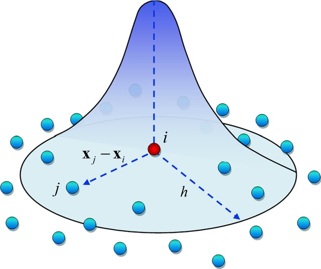
\includegraphics[width=\textwidth]{../../conference/images/kernel.png}
                \caption*{fonction noyau $\phi_h$}
            \end{figure}
        \end{column}
    \end{columns}
\end{frame}

%8
\begin{frame}{Mise à jour EnKF pour les simulations sans maillage}
    \begin{columns}[t]
        \begin{column}{0.7\textwidth}
            Correction des membres $i = 1, \dots, N_{\text{ens}}$ : \\
            \vspace{-0.50cm}
            \begin{eqnarray*}
                u_i^a(x) &=& u^f_i(x) + \sum_{j=1}^{N_{\text{ens}}} F_{ij}~u^f_j(x), \\
                &=& \sum_{p \in \mathcal{P}^f_i} \Gamma^f_p \phi_h(x - x_p) + \sum_{j=1}^{N_{\text{ens}}} F_{ij} \sum_{{p'} \in \mathcal{P}_j^f} \Gamma^f_{p'} \phi_h(x - x_{p'}), \\
                &=& \sum_{j=1}^{N_{\text{ens}}} \sum_{ p \in \mathcal{P}^f_i} \Gamma^a_p \phi_h (x - x_p)
            \end{eqnarray*}
            \vspace{-0.10cm}
            $\Rightarrow u_i^a$ est une combinaison de \textbf{toutes les particules}! \\
            \vspace{-0.10cm}
            \begin{equation*}
                \text{Card}(\mathcal P^a_i) = \sum_{j=1}^{N_{\text{ens}}}\text{Card}(\mathcal P^f_j)
            \end{equation*}
        \end{column}
        \begin{column}{0.3\textwidth}
            \vspace{-1cm}
            \begin{figure}
                \centering
                \begin{subfigure}{\textwidth}
                    \centering
                    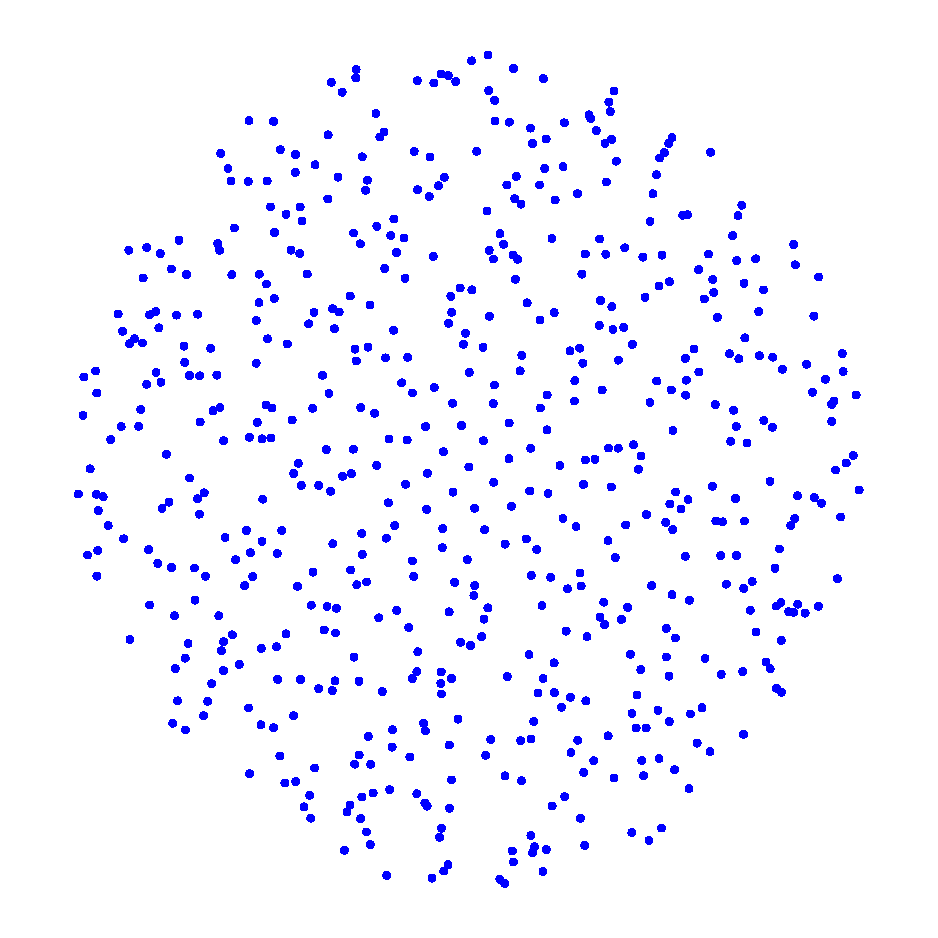
\includegraphics[width=0.7\textwidth]{../../conference/images/memb_particles.pdf}
                \end{subfigure}
                \begin{subfigure}{\textwidth}
                    \centering
                    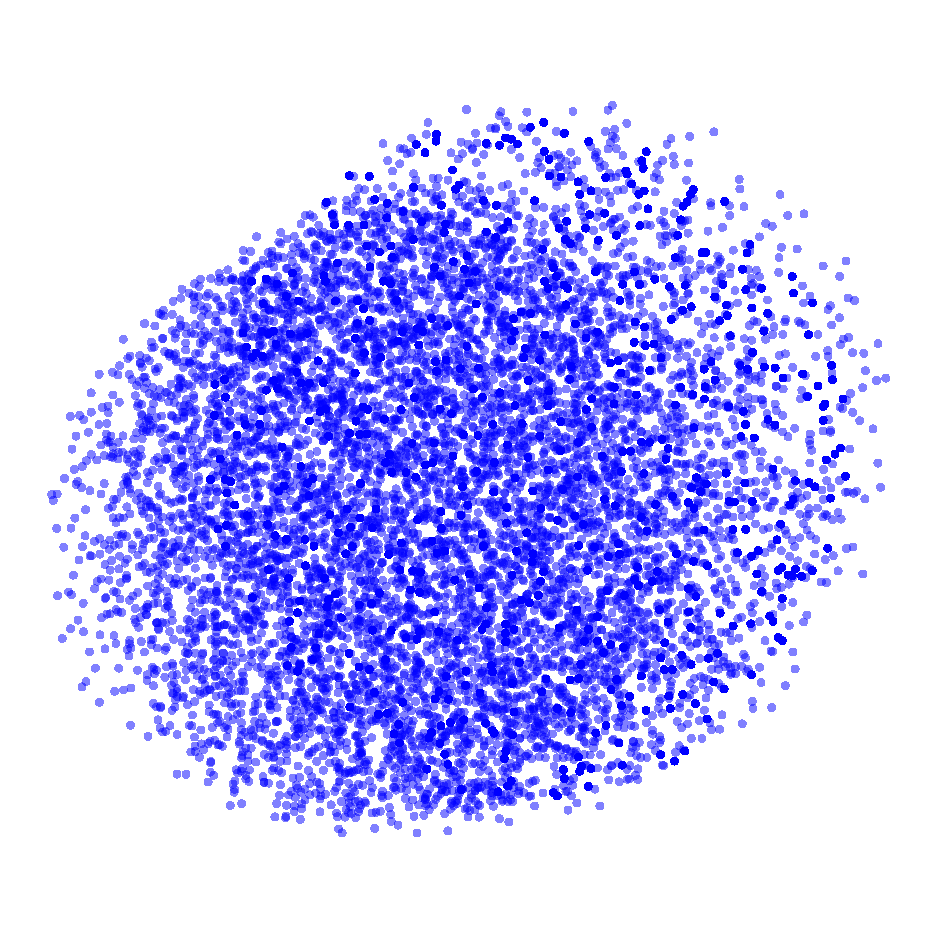
\includegraphics[width=0.7\textwidth]{../../conference/images/all_particles.pdf}
                \end{subfigure}
                \caption*{Support des particules avant et après la correction}
            \end{figure}
        \end{column}
    \end{columns}
\end{frame}

\section{Correction des intensités}
\begin{frame}{Correction des intensités}
    \small
    \textbf{Solution 1 - Remesh-EnKF} \\

    Générer un nouvel ensemble de particules régulières avec un opérateur de grille de particules \\

    \begin{columns}
        \begin{column}{0.6\textwidth}
            Mise à jour en deux étapes :
            \begin{itemize}
                \item Pour chaque membre $i$, générer un nouvel ensemble régulier de particules avec un schéma de redistribution pour obtenir des positions communes~\footnotemark[1]
                      \begin{equation*}
                          \Gamma^f_{g, i} = \sum_{p \in \mathcal P^i} \Gamma^f_{p, i} W(\frac{x_{p, i} - z_g}{h}), \quad g \in \mathcal G,
                      \end{equation*}
                      avec $W$ le noyau de remeshing,
                \item Mettre à jour les intensités des particules au même endroit
                      \begin{equation*}
                          \Gamma^a_{g, i} = \Gamma^f_{g, i} + \sum_{j=1}^{N_{\text{ens}}} F_{ij} \Gamma^f_{g,j}
                      \end{equation*}
            \end{itemize}
        \end{column}
        \hspace{-0.2cm}
        \begin{column}{0.3\textwidth}
            \begin{figure}
                \only<1>{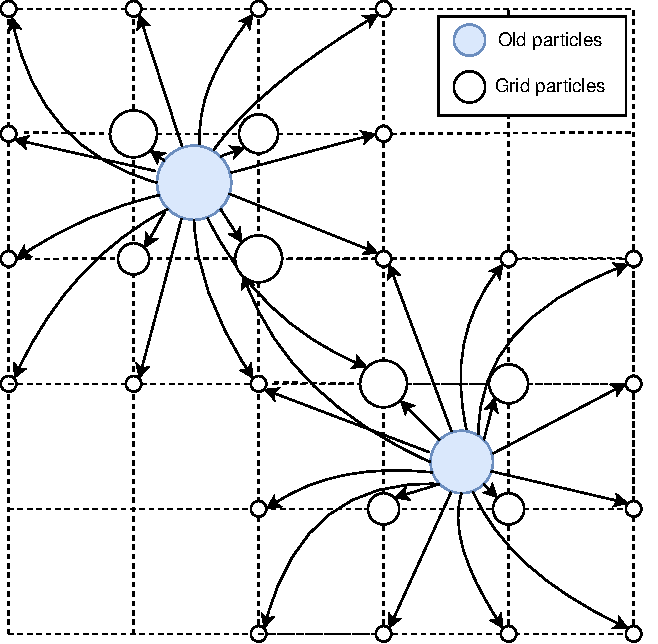
\includegraphics[width=\textwidth]{../../conference/images/redistribution.pdf}}
                \only<2>{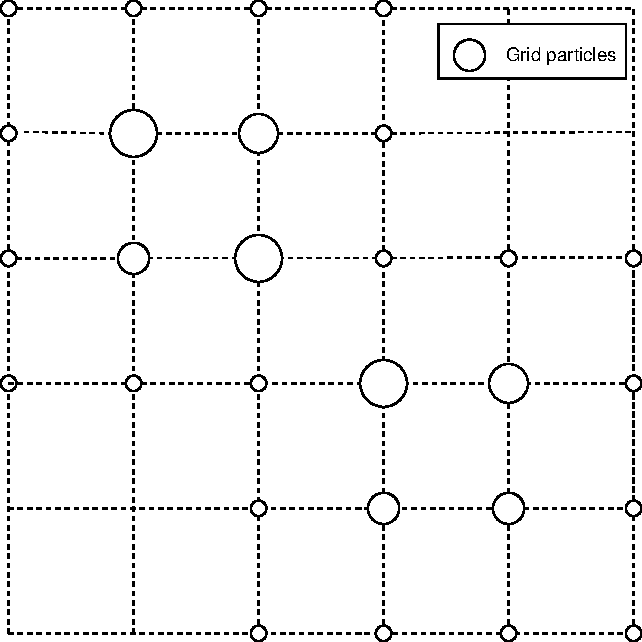
\includegraphics[width=\textwidth]{../../conference/images/redistribution_grid.pdf}}
                \only<3>{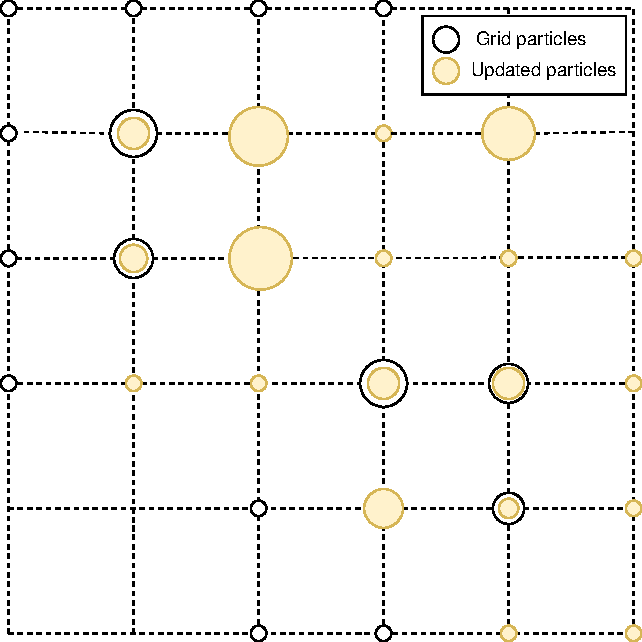
\includegraphics[width=\textwidth]{../../conference/images/redistribution_update.pdf}}
                \only<4>{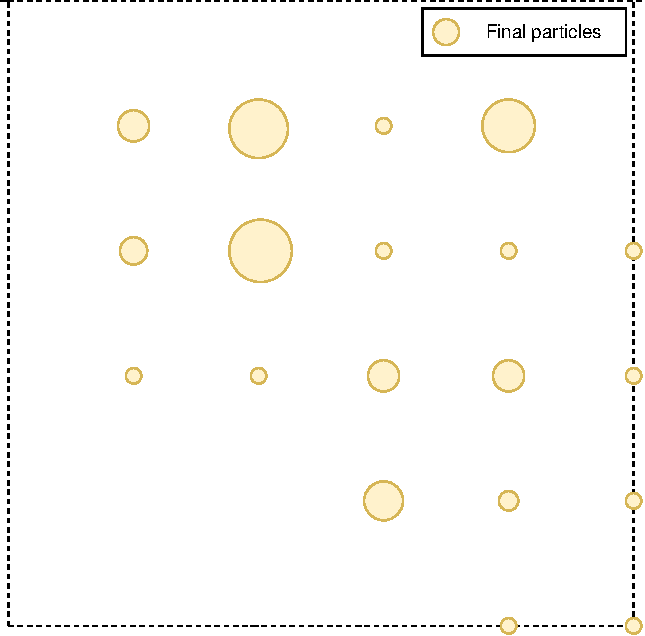
\includegraphics[width=\textwidth]{../../conference/images/redistribution_final.pdf}}
            \end{figure}
        \end{column}
    \end{columns}

    \footnotetext[1]{\tiny utilisé par les méthodes \textit{Particle-In-Cell} (MPM, VIC,...).}
\end{frame}

\begin{frame}{Correction des intensités}
    \small
    \textbf{Solution 2 - Part-EnKF} \\
    Conserver le même ensemble de positions de particules \\
    \begin{columns}[t]
        \begin{column}{0.6\textwidth}
            \begin{eqnarray*}
                u_i^f(x) &=& \sum_{p \in \mathcal P_i} \textcolor{ceared}{\Gamma^f_p} \phi_h(x - x_p^f),\\
                \quad u^a_i(x) &=& u_i^f(x) + \sum_{j=1}^{N_{\text{ens}}} F_{ij} u_j^f(x) \approx \sum_{p \in \mathcal P_i} \textcolor{ceared}{\Gamma^a_p} \phi_h(x - x_p^f), \\
            \end{eqnarray*}
        \end{column}

        \begin{column}{0.4\textwidth}
            \vspace{-0.8cm}
            \begin{figure}
                \only<1>{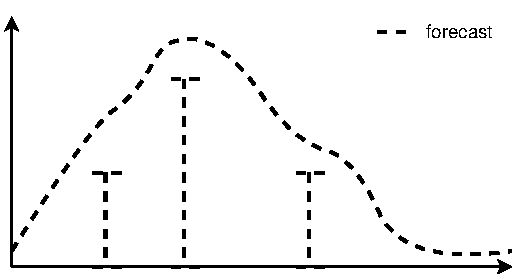
\includegraphics[width=\textwidth]{../../conference/images/forecast_part.pdf}}
                \only<2>{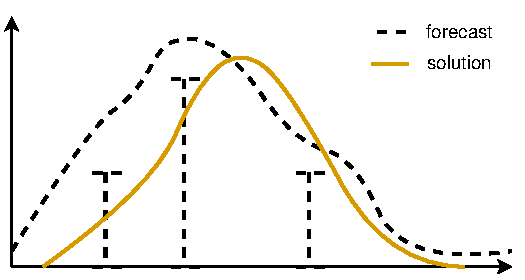
\includegraphics[width=\textwidth]{../../conference/images/with_solution.pdf}}
                \only<3>{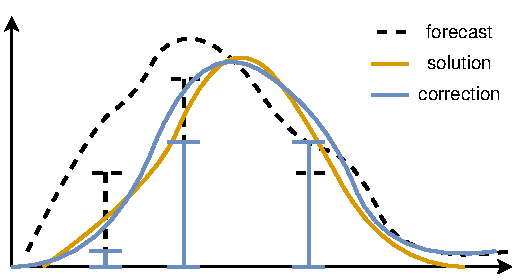
\includegraphics[width=\textwidth]{../../conference/images/correction_final.pdf}}
            \end{figure}
        \end{column}
    \end{columns}

    % \vspace{-0.8cm}
    \begin{columns}[t]
        \begin{column}{0.4\textwidth}
            \begin{exampleblock}{Approximation particulaire}
                $\Gamma^a_p = \int_{\Omega_p} u^a_i(x) dV \approx u^a_i(x_p) V_p$
            \end{exampleblock}
        \end{column}
        \begin{column}{0.6\textwidth}
            \begin{exampleblock}{Régression RBF}
                \begin{eqnarray*}
                    u^a_i(x_p) &\approx& \sum_{p' \in \mathcal P_i} \Gamma^a_{p'} \phi_h(x_p - x_{p'}), \quad p \in \mathcal P_i \Rightarrow \bm u_i \approx \Phi \bm \Gamma_i\\
                    \Rightarrow \bm \Gamma_i^a &=& \argmin_{\bm \Gamma \in \mathbb R^{N_p}} \| \bm u_i - \Phi \bm \Gamma\|_2^2 + R(\bm \Gamma)
                \end{eqnarray*}
            \end{exampleblock}
        \end{column}
    \end{columns}
\end{frame}

%10
\begin{frame}{Un exemple simplifié: méthode vortex~\footnotemark[1]}
    \small
    \vspace{-0.5cm}
    \begin{columns}[t]
        \begin{column}{0.5\textwidth}
            \begin{itemize}
                \item équation de Navier-Stokes incompressible: discrétisation du champ de tourbillon \textbf{vorticity field} $\omega(x, t)$ \\
                      \begin{eqnarray*}
                          \frac{\partial \bm \omega}{\partial t} + (\bm{v} \cdot \nabla) \bm \omega - \nu \Delta \bm \omega & = 0, \\
                          \nabla \cdot \bm v                                                                                & = 0,
                      \end{eqnarray*}
                \item l'intensité $\Gamma_p$ est une \textbf{circulation} locale
                \item Modèle d'évolution : \\
                      \begin{eqnarray*}
                          \frac{d\Gamma_p}{dt} &=& \nu \varepsilon^{-2} \sum_q (\Gamma_q - \Gamma_p) \eta_\varepsilon(x_q - x_p), \\
                          \frac{d x_p}{d t} &=& v(x_p; \mathcal P) \\
                          &=& \sum_{p' \in \mathcal P} \Gamma_{p'} \vec{V}(x_p - x_{p'}) + v_{BC} \\
                      \end{eqnarray*}
            \end{itemize}
            \footnotetext[1]{\tiny \cite{cottet_vortex_2000}}
        \end{column}
        \begin{column}{0.5\textwidth}
            %mettre les deux images
            \begin{figure}
                \animategraphics[loop, autoplay, width=0.85\textwidth]{10}{../../conference/images/dipole_particles/dipole_particles-}{0}{35}%
            \end{figure}
        \end{column}
    \end{columns}
\end{frame}

\subsection{Application - dipôle de Lamb–Chaplygin}
%11.1 presenter le dipole
\begin{frame}{Application - dipôle de Lamb–Chaplygin}
    Dipôle se translatant à la vitesse $U$
    \begin{columns}
        \begin{column}{0.33\textwidth}
            \animategraphics[loop, autoplay, width=0.85\textwidth]{10}{../../conference/images/dipole_estimate/ensemble_dipole/ensemble_dipole-}{0}{27}%
        \end{column}
        \begin{column}{0.66\textwidth}
            \animategraphics[loop, autoplay, width=0.85\textwidth]{10}{../../conference/images/dipole_estimate/ensemble_estimate/ensemble_estimate-}{0}{27}%
        \end{column}
    \end{columns}
\end{frame}

%11.3 présenter la correction
\begin{frame}{Application - assimilation}
    \begin{figure}[t]
        \centering
        \begin{subfigure}{0.3\textwidth}
            \centering
            \alt<2>{%
                \animategraphics[loop, autoplay, height=0.3\textheight]{10}{../../conference/images/dipole_estimate/reference/reference-}{0}{40}}
            {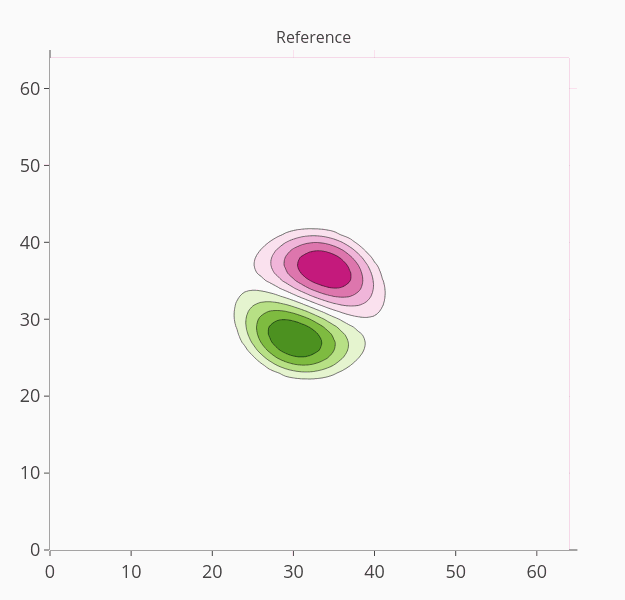
\includegraphics[height=0.3\textheight]{../../conference/images/dipole_estimate/reference/reference-0.png}}
            \caption*{\tiny référence}
        \end{subfigure}
        \begin{subfigure}{0.3\textwidth}
            \centering
            \alt<2>{%
                \animategraphics[loop, autoplay, height=0.3\textheight]{10}{../../conference/images/dipole_estimate/obs_no_noise/obs_no_noise-}{0}{19}}
            {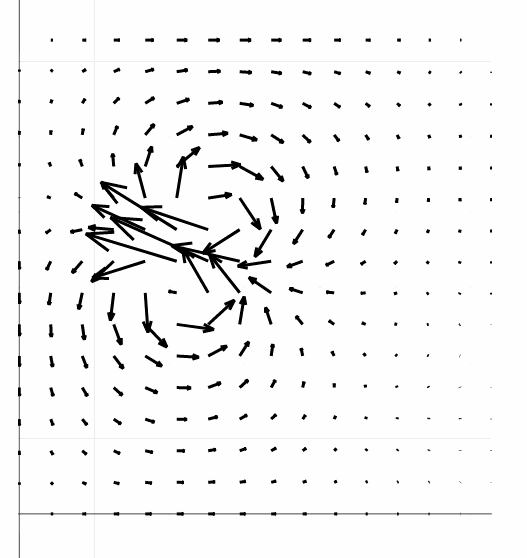
\includegraphics[height=0.3\textheight]{../../conference/images/dipole_estimate/obs_no_noise/obs_no_noise-0.png}}
            \caption*{\tiny champ vitesse}
        \end{subfigure}
        \begin{subfigure}{0.3\textwidth}
            \centering
            \alt<2>{%
                \animategraphics[loop, autoplay, height=0.3\textheight]{10}{../../conference/images/dipole_estimate/obs_noise/obs_noise-}{0}{19}}
            {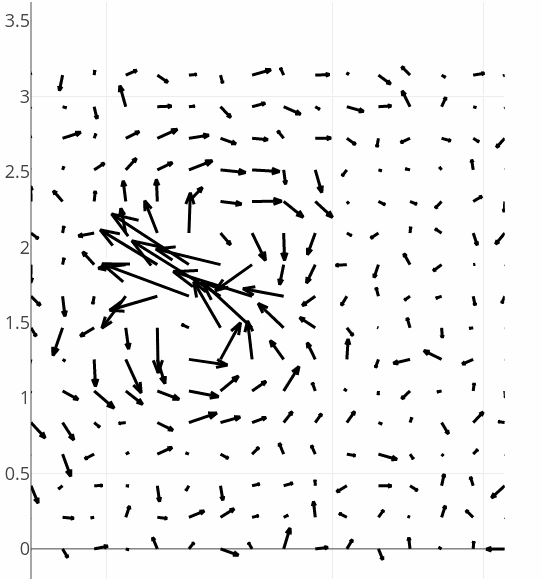
\includegraphics[height=0.3\textheight]{../../conference/images/dipole_estimate/obs_noise/obs_noise-0.png}}
            \caption*{\tiny champ vitesse bruité}
        \end{subfigure}
    \end{figure}
    \begin{figure}[t]
        \begin{subfigure}{0.3\textwidth}
            \centering
            \alt<2>{%
                \animategraphics[loop, autoplay, height=0.3\textheight]{10}{../../conference/images/dipole_estimate/estimate/estimate-}{0}{40}}
            {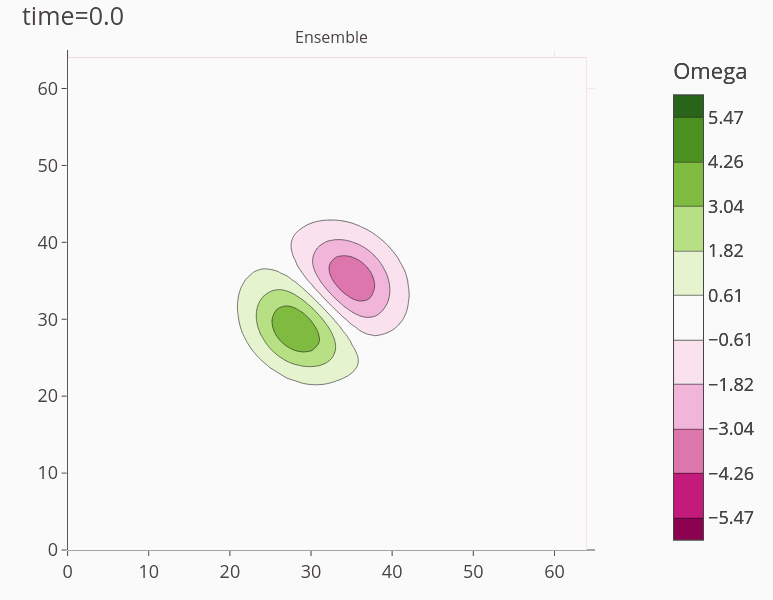
\includegraphics[height=0.3\textheight]{../../conference/images/dipole_estimate/estimate/estimate-0.png}}
            \caption*{\tiny estimateur}
        \end{subfigure}
        \begin{subfigure}{0.3\textwidth}
            \centering
            \alt<2>{%
                \animategraphics[loop, autoplay, height=0.3\textheight]{10}{../../conference/images/dipole_estimate/ensemble_sample/ensemble_sample-}{0}{40}}
            {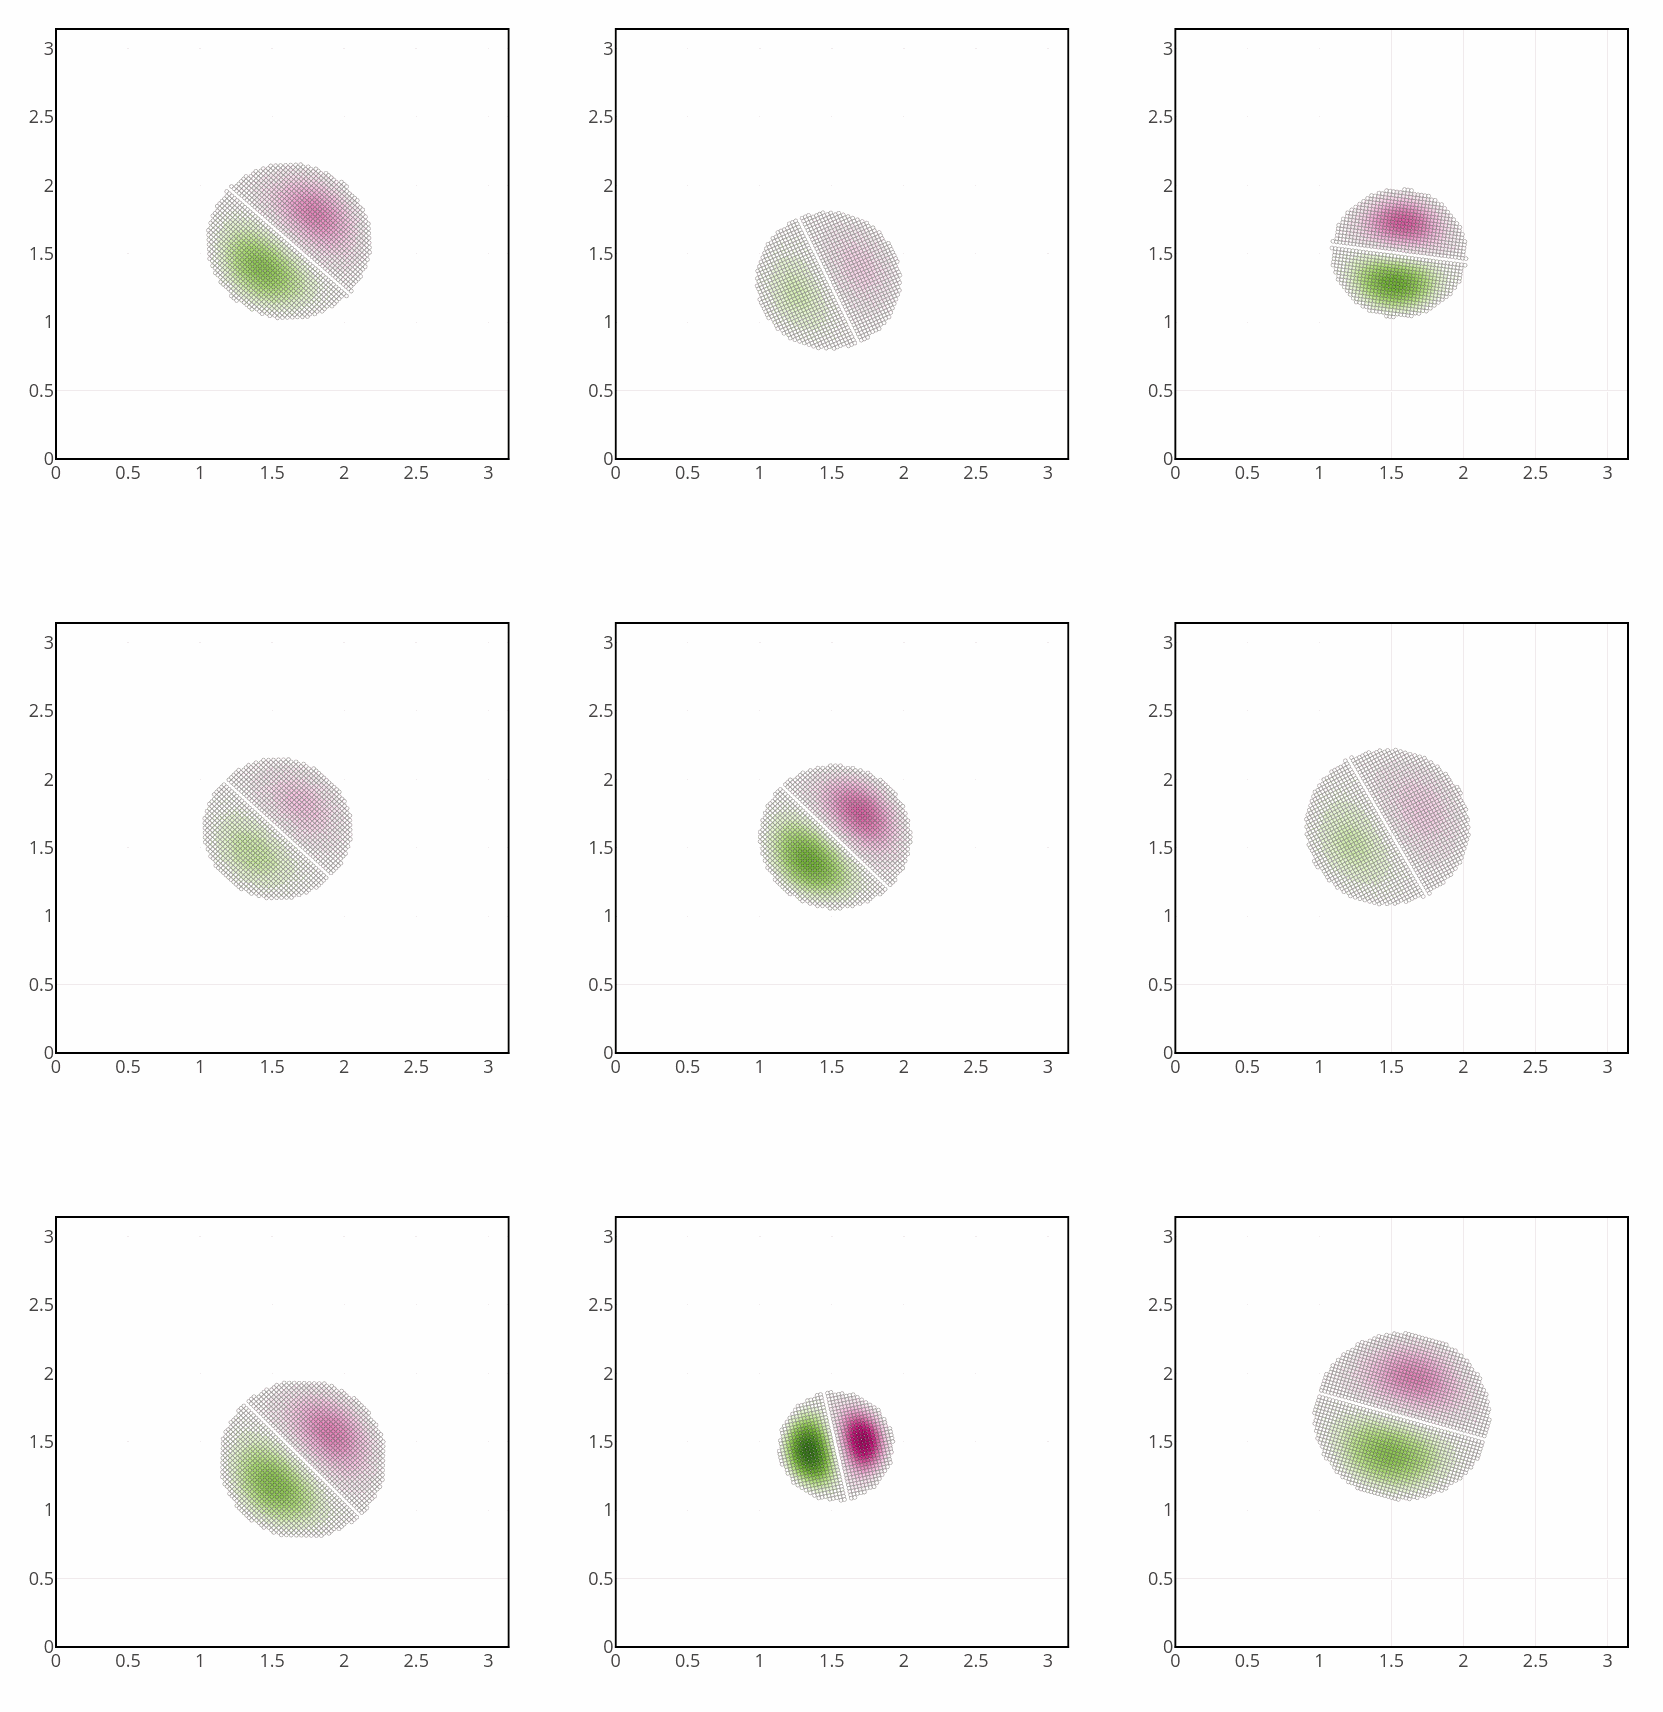
\includegraphics[height=0.3\textheight]{../../conference/images/dipole_estimate/ensemble_sample/ensemble_sample-0.png}}
            \caption*{\tiny échantillons}
        \end{subfigure}
        \hfill
    \end{figure}
\end{frame}

%11.4 présenter les courbes 
\begin{frame}{Comparaison}
    \begin{columns}[t]
        \begin{column}{0.33\textwidth}
            \begin{figure}
                \begin{subfigure}{\textwidth}
                    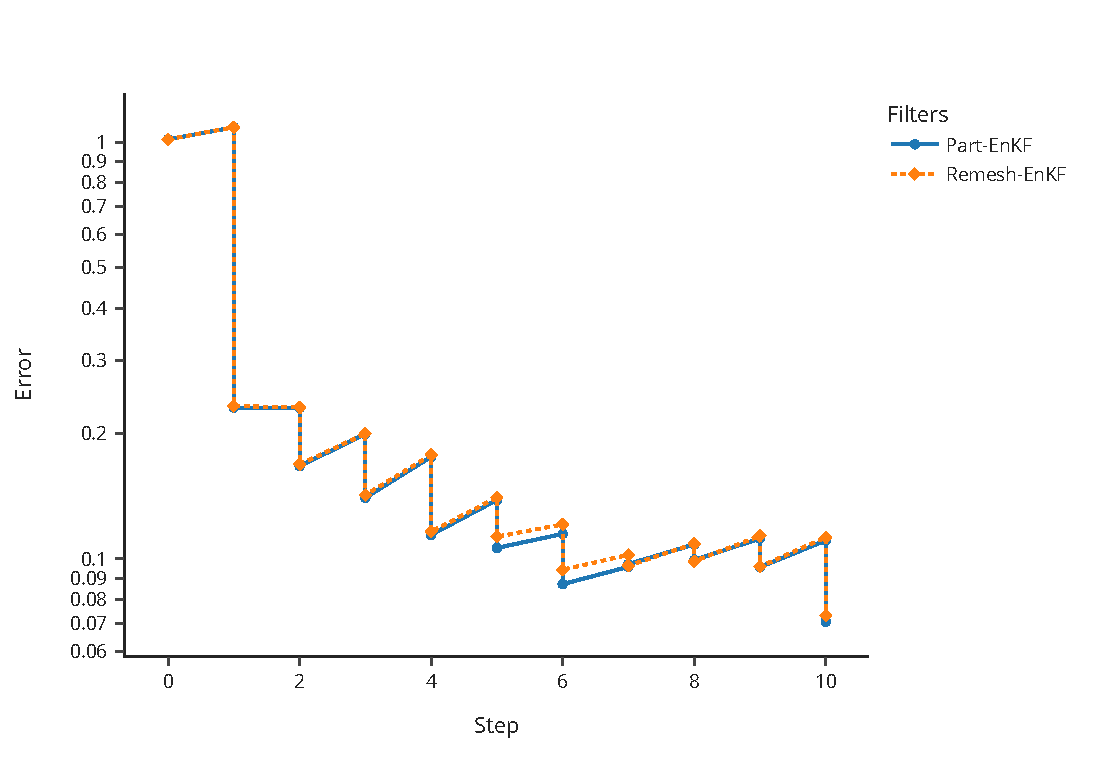
\includegraphics[width=\textwidth]{../../conference/images/dipole_results/error_in_time.pdf}
                \end{subfigure}
                \begin{subfigure}{\textwidth}
                    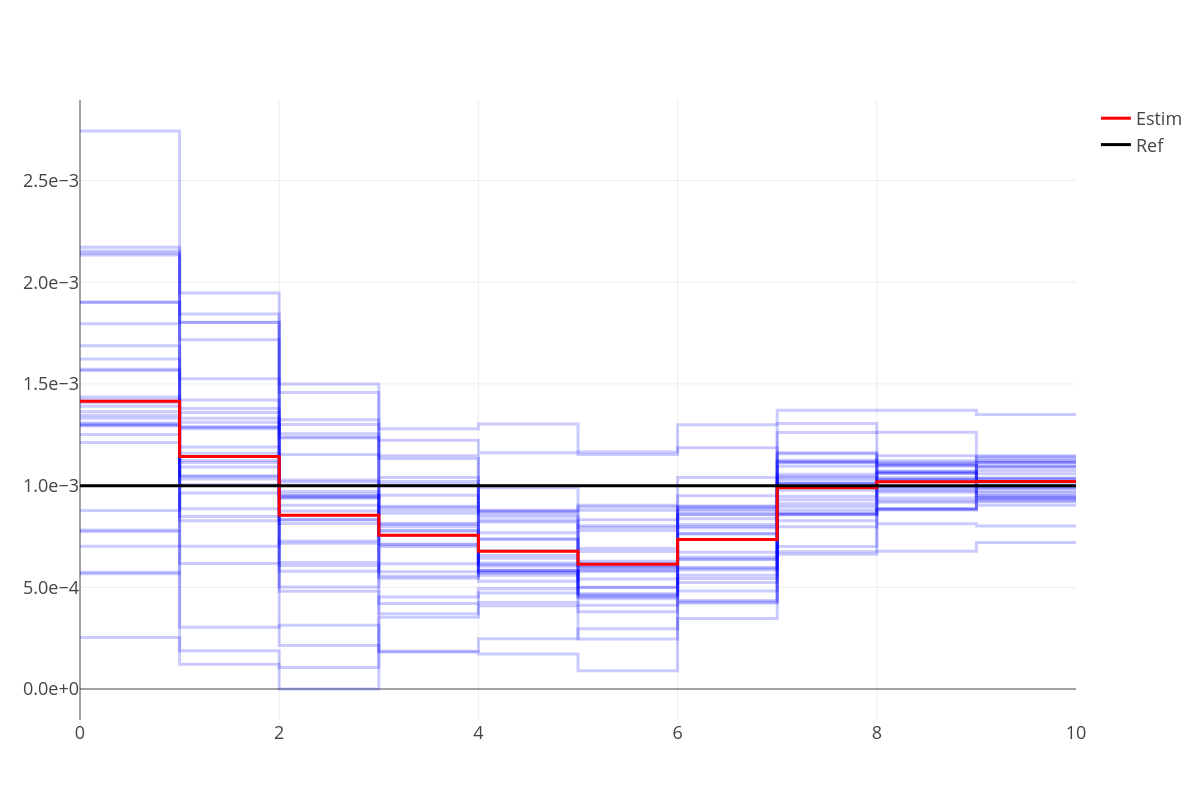
\includegraphics[width=\textwidth]{../../conference/images/dipole_results/visc_rmf.png}
                \end{subfigure}
            \end{figure}
        \end{column}
        \begin{column}{0.33\textwidth}
            \begin{figure}
                \begin{subfigure}{\textwidth}
                    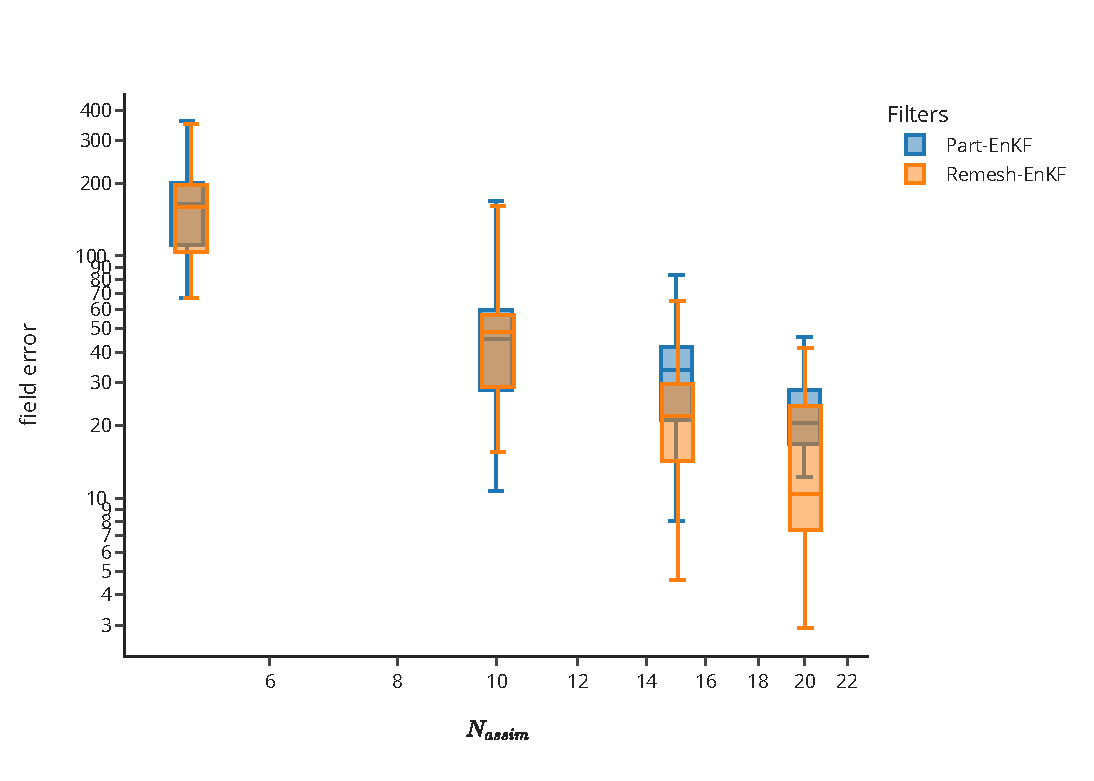
\includegraphics[width=\textwidth]{../../conference/images/dipole_results/MSE_na_box_log_log.pdf}
                \end{subfigure}
                \begin{subfigure}{\textwidth}
                    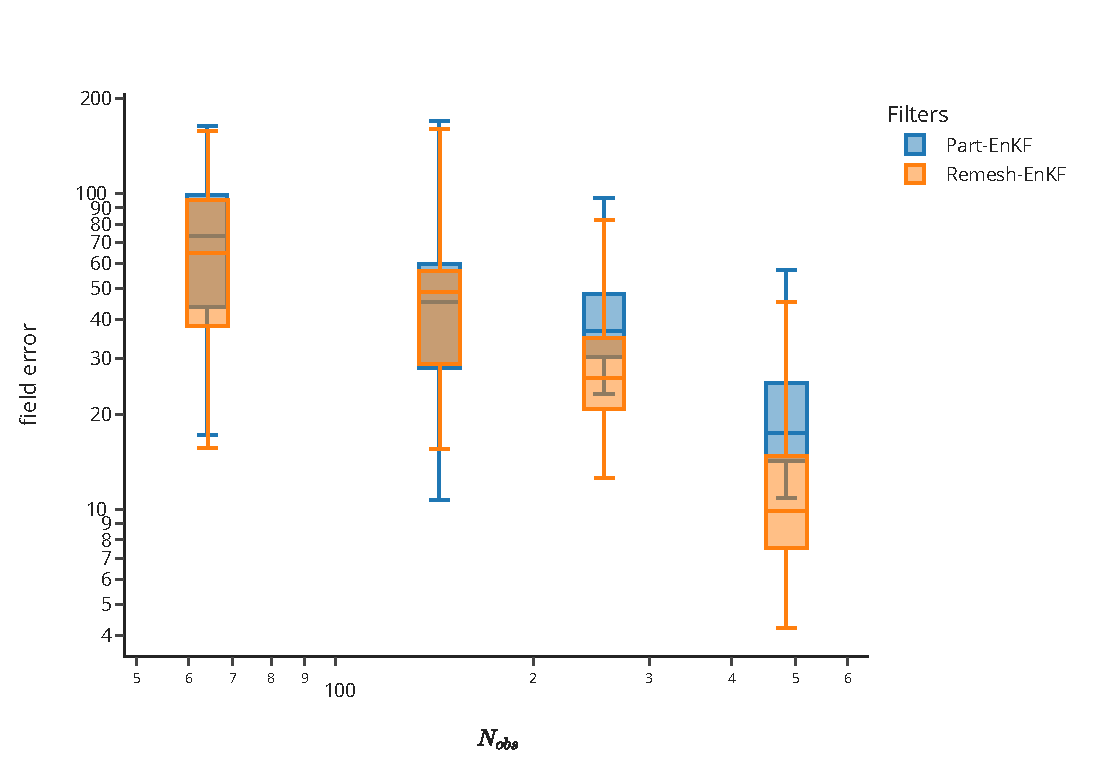
\includegraphics[width=\textwidth]{../../conference/images/dipole_results/MSE_nobs_box_log_log.pdf}
                \end{subfigure}
            \end{figure}
        \end{column}
        \begin{column}{0.33\textwidth}
            \begin{figure}
                \begin{subfigure}{\textwidth}
                    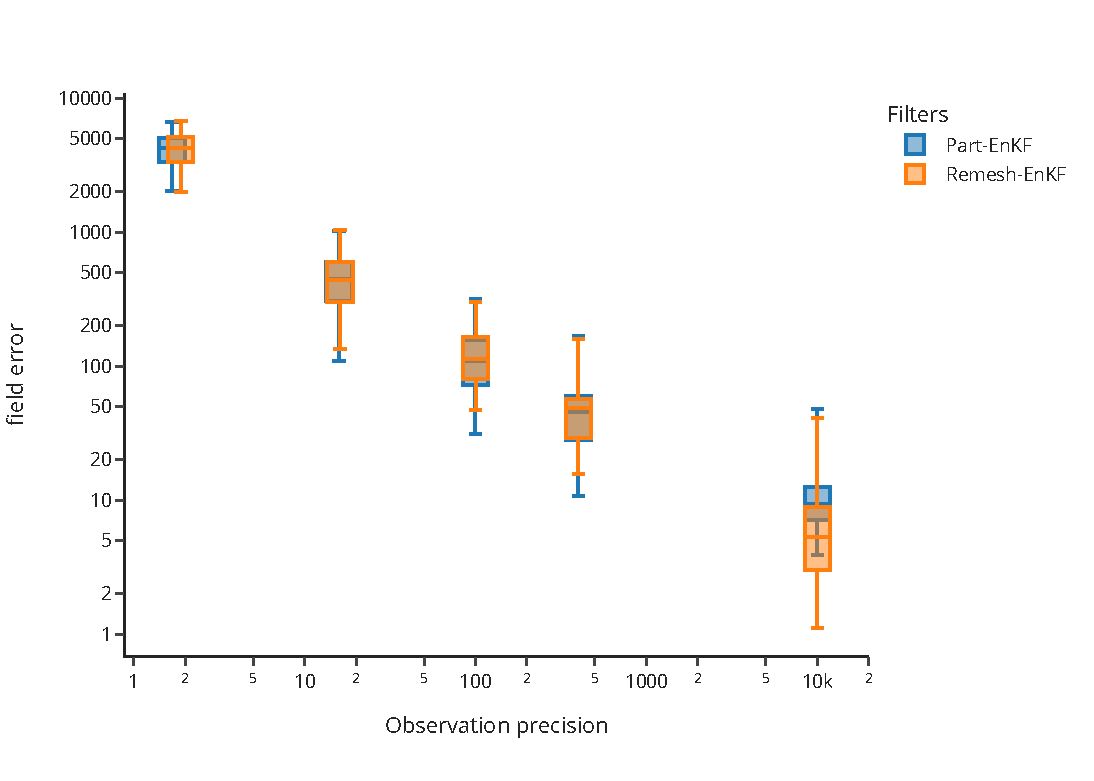
\includegraphics[width=\textwidth]{../../conference/images/dipole_results/MSE_obs_precision_box_log.pdf}
                \end{subfigure}
                \begin{subfigure}{\textwidth}
                    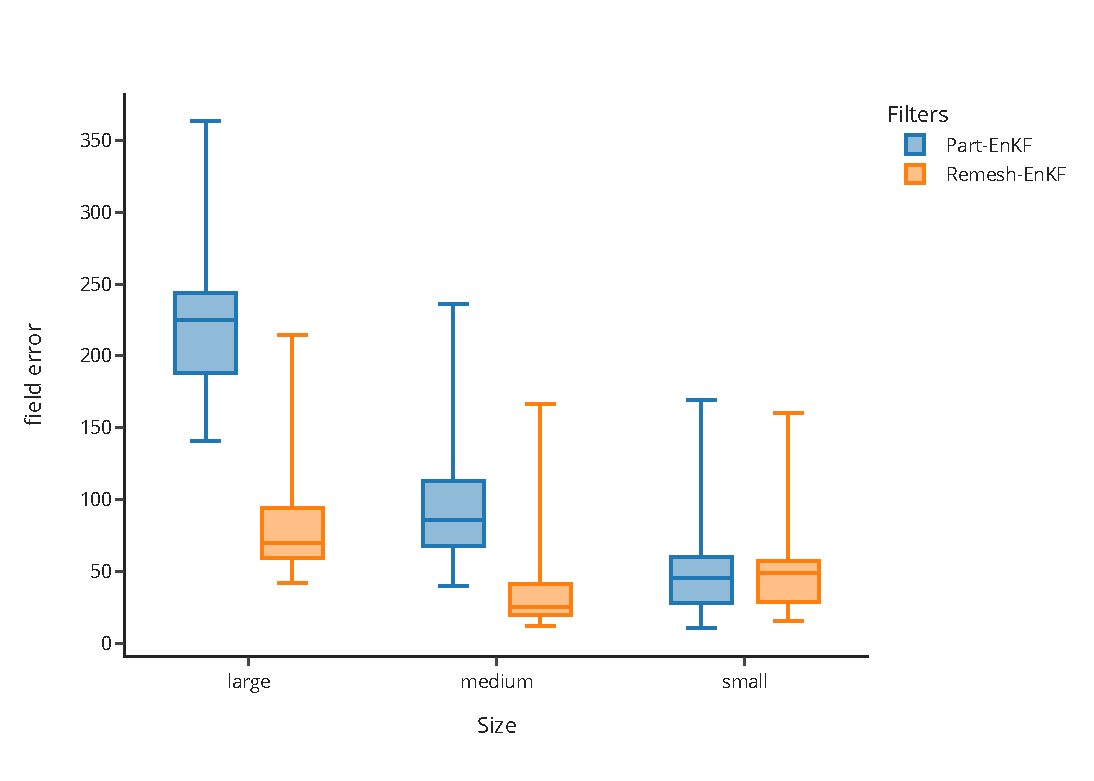
\includegraphics[width=\textwidth]{../../conference/images/dipole_results/MSE_size_box.pdf}
                \end{subfigure}
            \end{figure}
        \end{column}
    \end{columns}
\end{frame}

%12
\begin{frame}{Part-EnKF - Limitation}
    Confiné au support des particules $\Rightarrow$ pourrait être inadéquat pour la solution analysée
    \begin{figure}
        \centering
        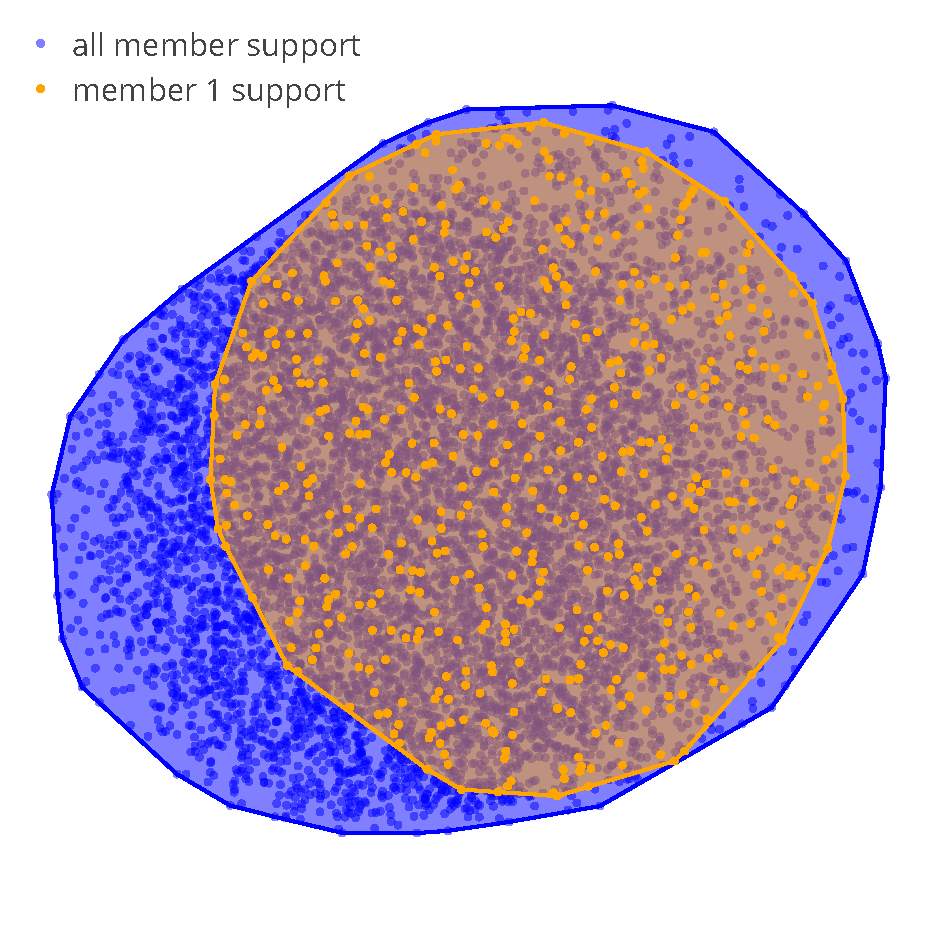
\includegraphics[width=0.4\textwidth]{../../conference/images/ens_particles.pdf}
    \end{figure}
\end{frame}

%13
\section{Correction de position}
\transition[3]{Assimilation par alignement}{correction de position}

\begin{frame}{Correction de position}
    \vspace{-0.9cm}
    \begin{eqnarray*}
        u_i^f(x) &=& \sum_{p \in \mathcal P_i} \Gamma^f_p \phi_h(x - \textcolor{ceared}{x_p^f}), \quad u^a_i(x) = u_i^f(x) + \sum_{j=1}^{N_{\text{ens}}} F_{ij} u_j^f(x), \\
        u_i^a(x) &\approx& \sum_{p \in \mathcal P_i} \Gamma^f_p \phi_h(x - \textcolor{ceared}{A_i(x_p^f)}), \\
    \end{eqnarray*}
    \vspace{-0.7cm}

    \begin{columns}[t]
        \begin{column}{0.6\textwidth}
            $A_i$ est une transformation $x^a_{p} = A_i(x^f_{p})$. \\
            On choisit~\footnotemark[1] d'écrire $A(x)$ comme la solution de\\
            \begin{equation*}
                \begin{cases}
                    x'(\tau = 0) = x,                                           \\
                    \frac{d x'}{d \tau} = w_i (x'), \quad A_i(x) = x'(\tau = 1) \\
                \end{cases}
            \end{equation*}avec $w_i$ un champ de vitesse \textbf{à définir}
        \end{column}
        \begin{column}{0.4\textwidth}
            \vspace{-2cm}
            \begin{figure}
                \centering
                \only<1>{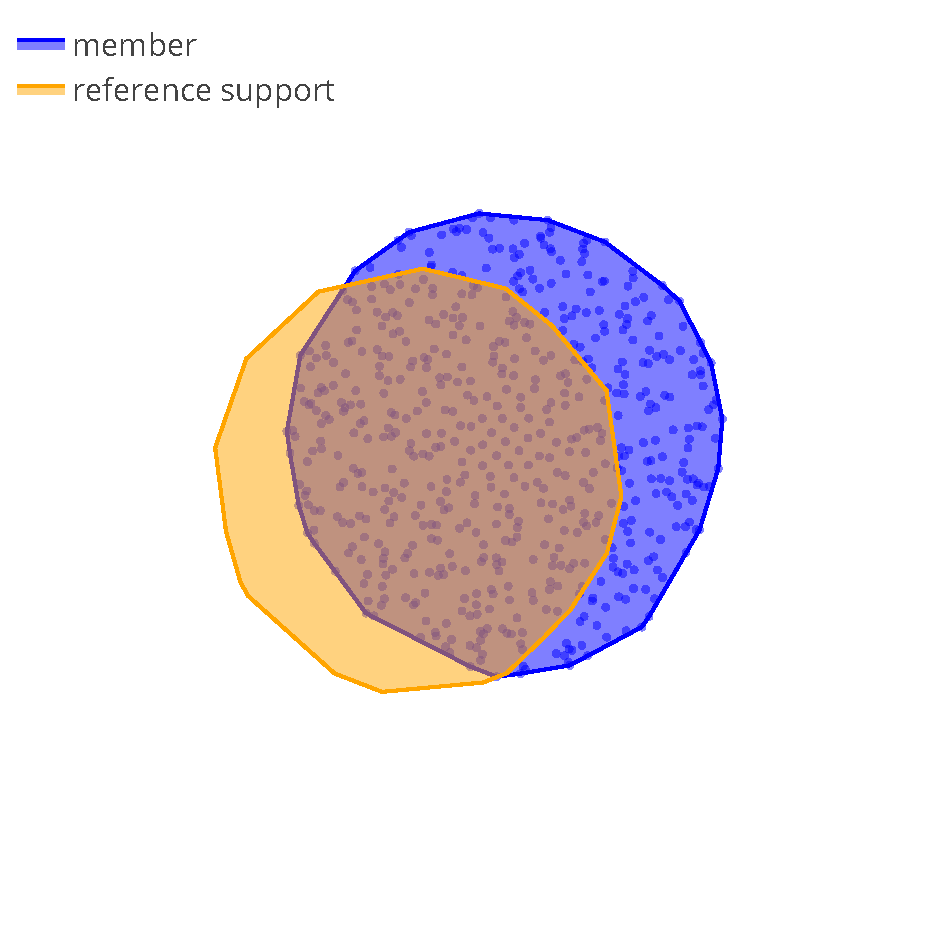
\includegraphics[width=0.8\textwidth]{../../conference/images/align_member_0.pdf}}
                \only<2>{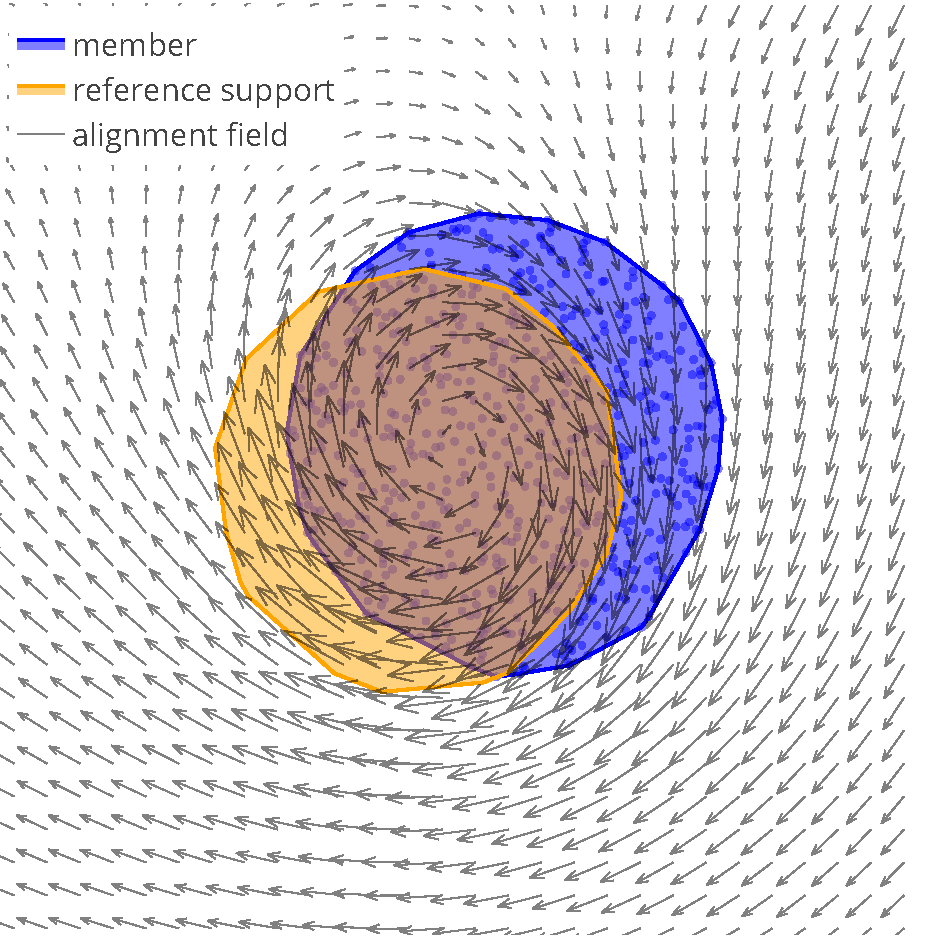
\includegraphics[width=0.8\textwidth]{../../conference/images/align_member_1.pdf}}
                \only<3>{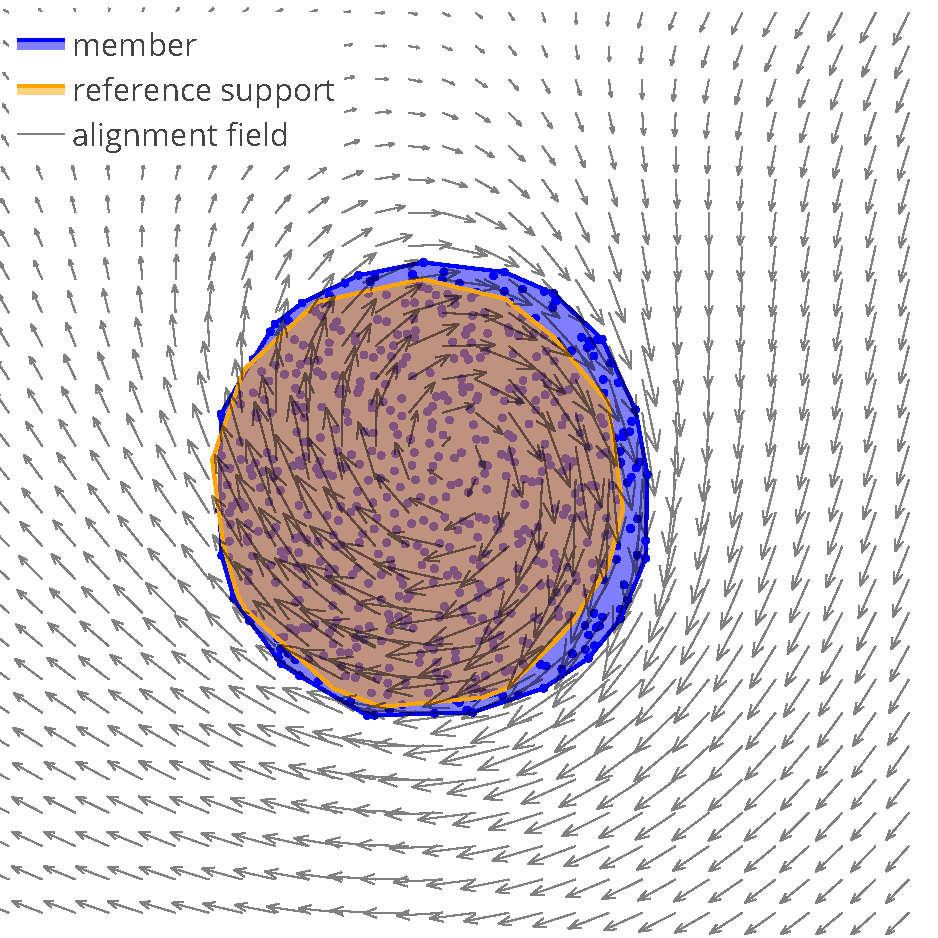
\includegraphics[width=0.8\textwidth]{../../conference/images/align_member_2_1.pdf}}
            \end{figure}
        \end{column}
    \end{columns}
    \vfill
    \footnotetext[1]{\tiny Other hypothesis have been made see~\cite{ravela_data_2007,rosenthal_displacement_2017}}
\end{frame}

\begin{frame}{Choix de $w_i$}
    Pour le membre $i$, on cherche à réduire l'écart entre les \textbf{prédictions} et les \textbf{observations}:
    \begin{equation*}
        w_i = \argmin_{w_i \in \mathcal V} \left\|y - \mathcal H(\mathcal{P}_i^f \mid w_i) \right\|^2_{R^{-1}} \visible<2->{\textcolor{ceared}{+ R(w)}}, \quad i = 1, \dots, N_{\text{ens}}
    \end{equation*}with $\mathcal V$ l'espace de recherche, $\mathcal H(\mathcal{P}_i^f \mid w_i)$ l'opérateur d'observation conditionné par $w_i$\\
    \vfill
    \visible<2->{\textcolor{ceared}{$R(w)$} est un terme de régularisation (éviter un mauvais conditionnement ou la non unicité)\\}
    \vfill
    \visible<2->{problème défini sur un espace \textbf{infini}}
    \vfill
\end{frame}

\begin{frame}{Formulation d'ordre réduit}

    On cherche le champ d'alignement comme la combinaison linéaire des champs de vitesse des membres,\\
    find $\bm a_i \in \mathbb{R}^{N_{\text{ens}}}$ \\
    \begin{equation*}
        w_i = \sum_{j=1}^{N_{\text{ens}}} a_{i,j} v_j (x) = \sum_{j=1}^{N_{\text{ens}}} a^i_j \left(\sum_{p \in \mathcal P_j} \Gamma_p^f \vec{V}(x - x_p) + v_{j,BC} \right)
    \end{equation*}
    \vfill
    \visible<2->{$N_{\text{ens}}$ problèmes indépendants de dimension $N_{\text{ens}}$ \\
        \begin{equation*}
            \mathcal L_i (a) = \min_{a \in \mathbb{R}^{N_{\text{ens}}}} \left\|d - \mathcal H_a(\hat u^f_i; a)_2 \right\|^2_{R^{-1}} + \lambda \|a\|_2^2, \quad i = 1, \dots, N_{\text{ens}}
        \end{equation*}
        Optimisés avec un optimiseur par descente de gradient (BFGS)}
    \vfill

\end{frame}

%14-17
\subsection{Application - problème des trois tourbillons(corps)}
\begin{frame}{Problème des trois tourbillons(corps)}
    \vspace{-0.5cm}
    \begin{columns}[t]
        \begin{column}{0.45\textwidth}
            \begin{itemize}
                \item \scriptsize \textbf{Variables d'intérêt}: centre des tourbillons
                \item \scriptsize \textbf{Incertitude initiale}: centre des tourbillons, amplitude, taille de coeur,...
                \item \scriptsize \textbf{Trajectoires chaotiques}~\footnotemark[1]
                \item \scriptsize \textbf{observations}: Une grille de vitesse grossière et bruitée
            \end{itemize}
            \begin{figure}
                \centering
                \vspace{-0.25cm}
                % \only<2->{\caption*{\tiny Vortex normalized position error}}
                \includegraphics<3->[width=\textwidth]{../../conference/images/error_position_wo_assim.pdf}
            \end{figure}
            \vfill
        \end{column}
        \begin{column}{0.55\textwidth}
            \centering
            \begin{figure}[t]
                \centering
                \visible<2->{\tiny Trajectoire des centre de vortex après perturbation}
                \only<3->{%
                    \animategraphics[loop, autoplay, width=0.85\textwidth]{10}{../../conference/images/vortex_centers_disperse/vortex_centers_}{0}{36}%
                }
                \only<2>{%
                    \animategraphics[loop, autoplay, width=0.85\textwidth]{10}{../../conference/images/vortex_centers_ref/vortex_centers_}{0}{36}%
                }
                \only<1>{%
                    \animategraphics[loop, autoplay, width=0.7\textwidth]{5}{../../conference/images/particles_ref/particles_ref_}{0}{20}
                }
            \end{figure}
        \end{column}
    \end{columns}
    \vspace{-0.5cm}

    \footnotetext[1]{\tiny \cite{aref_motion_1979}}
\end{frame}

\begin{frame}{Remesh-EnKF}
    \begin{columns}[t]
        \begin{column}{0.5\textwidth}
            \vspace{-0.5cm}
            \begin{figure}
                \centering
                \animategraphics[loop, autoplay, width=\textwidth]{10}{../../conference/images/vortex_centers_remesh_enkf/vortex_centers_}{0}{36}
            \end{figure}
        \end{column}
        \begin{column}{0.5\textwidth}
            \begin{figure}
                \centering
                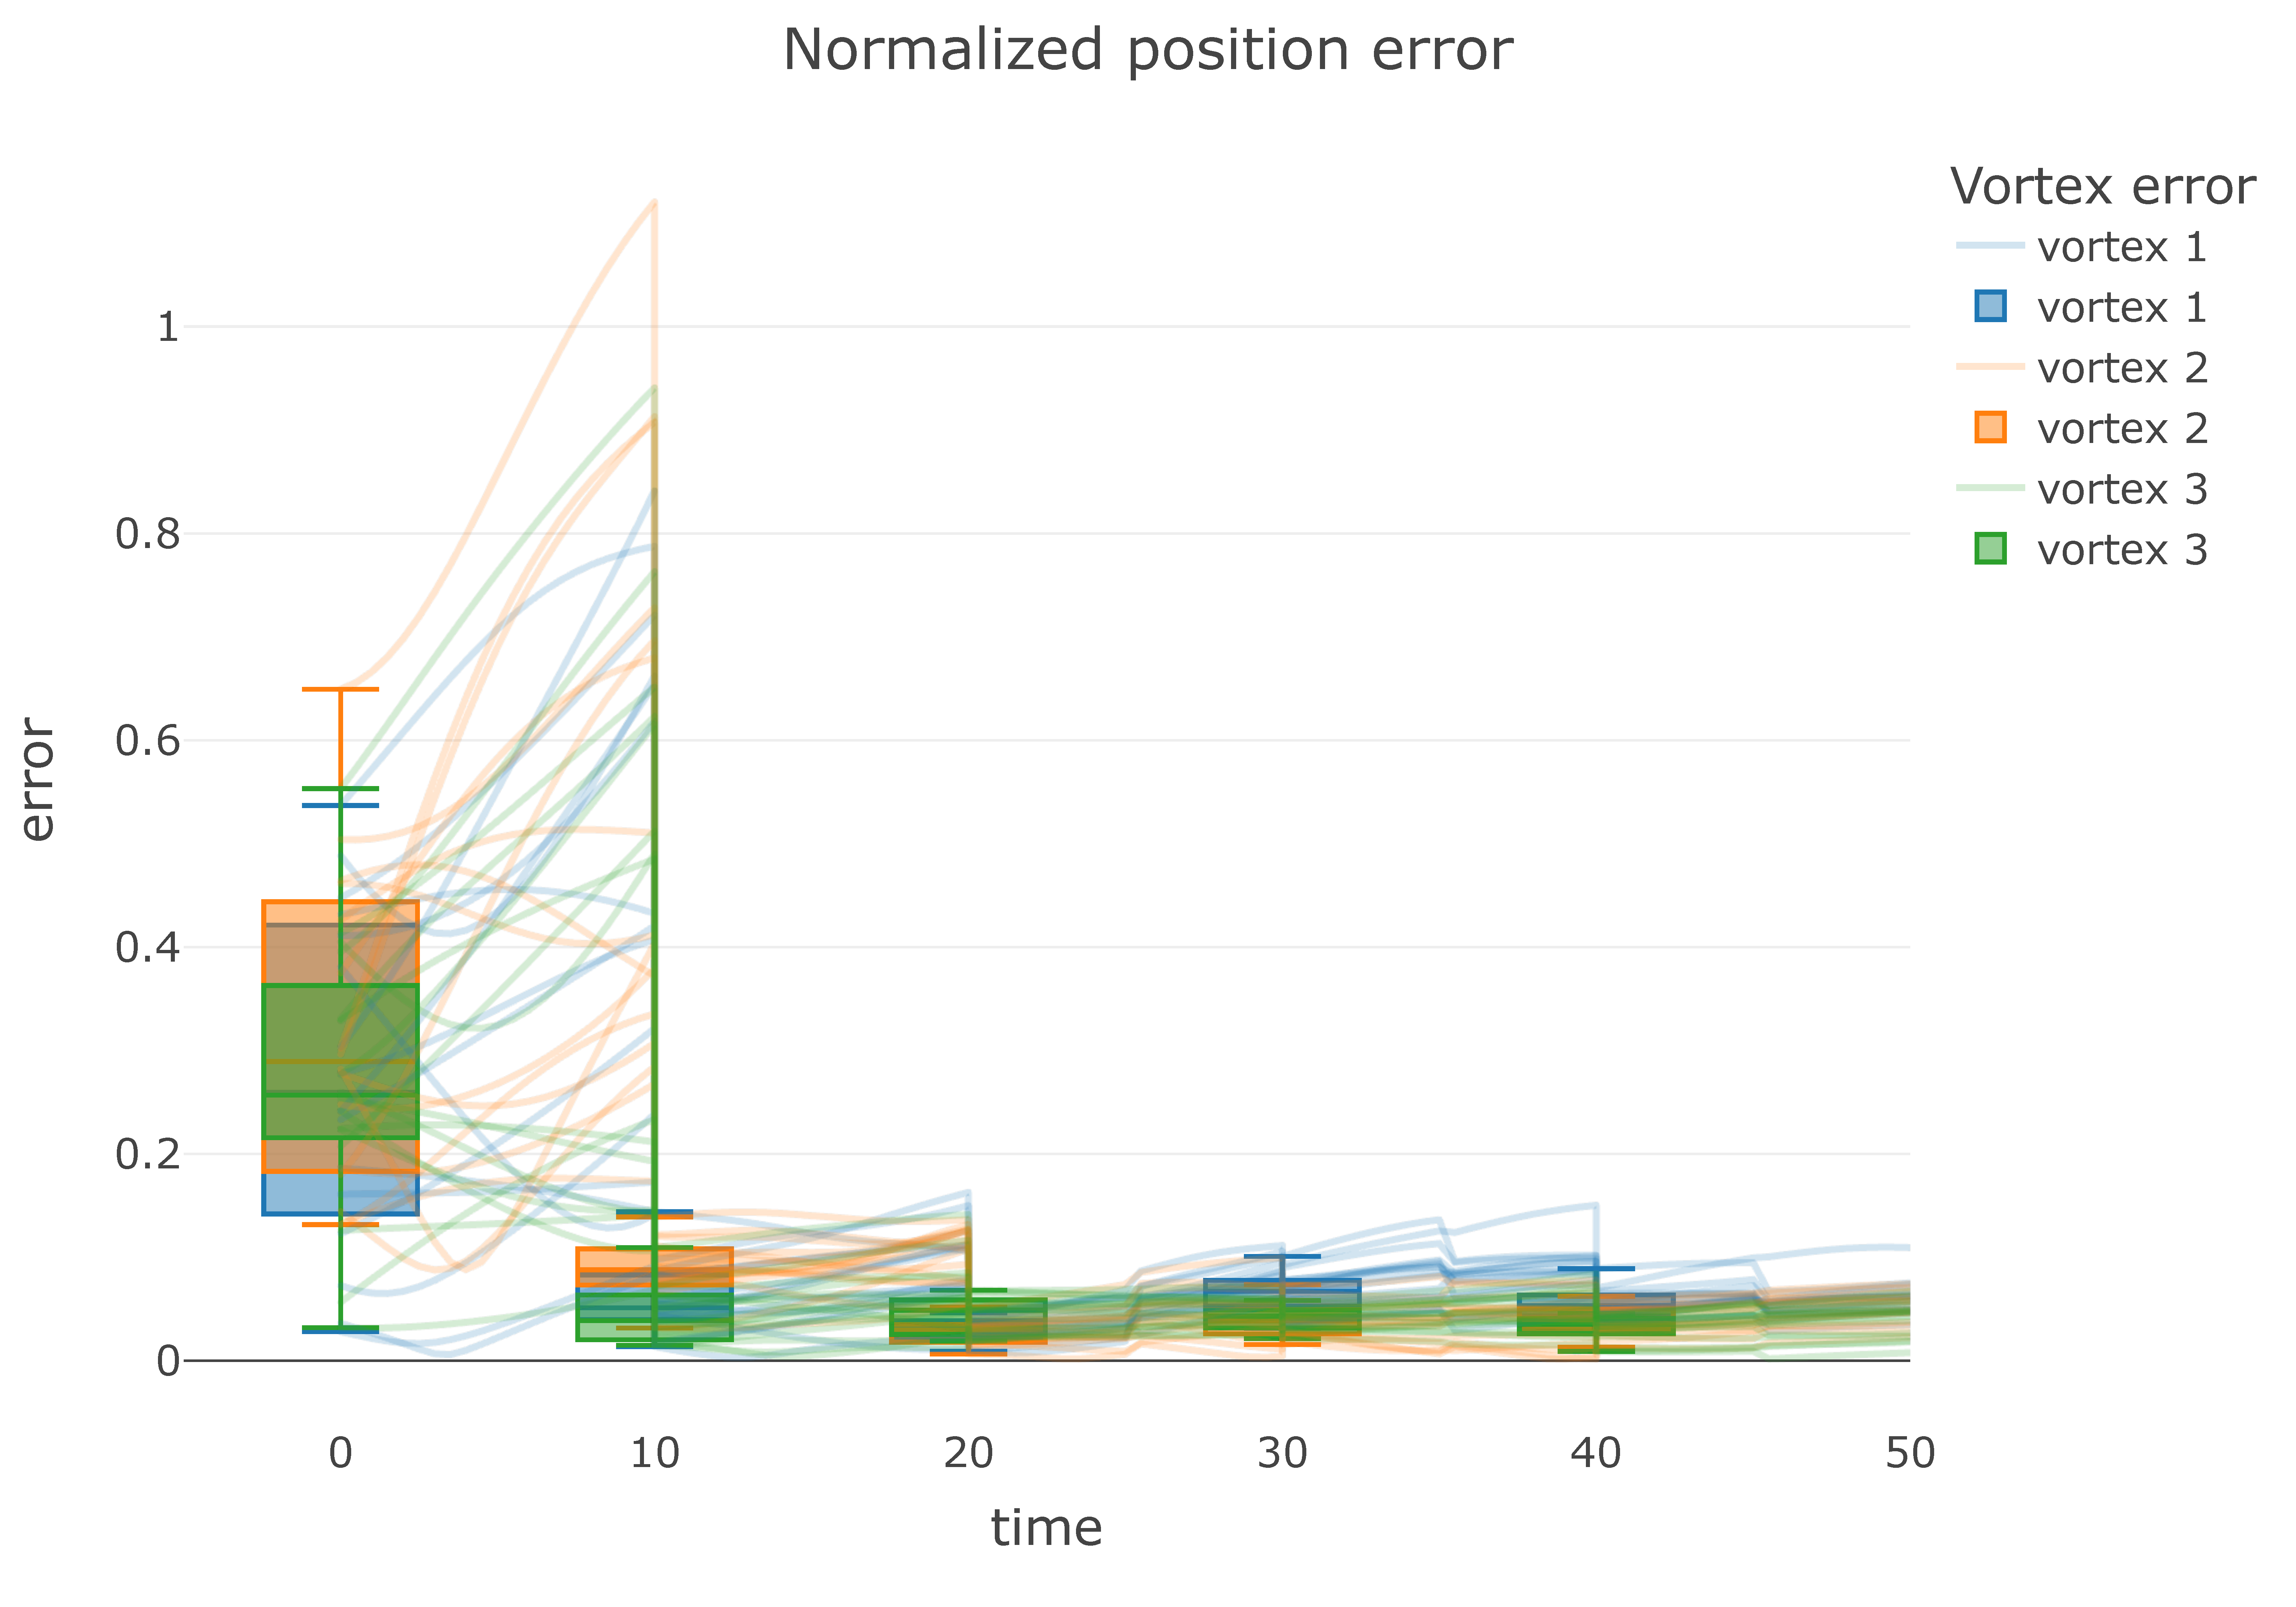
\includegraphics[width=\textwidth]{../../conference/images/remesh_enkf_error.pdf}
            \end{figure}
        \end{column}
    \end{columns}
\end{frame}

\begin{frame}{Part-EnKF}
    \begin{columns}[t]
        \begin{column}{0.5\textwidth}
            \vspace{-0.5cm}
            \begin{figure}
                \centering
                \animategraphics[loop, autoplay, width=\textwidth]{10}{../../conference/images/vortex_centers_part_enkf/vortex_centers_}{0}{36}
            \end{figure}
        \end{column}
        \begin{column}{0.5\textwidth}
            \begin{figure}
                \centering
                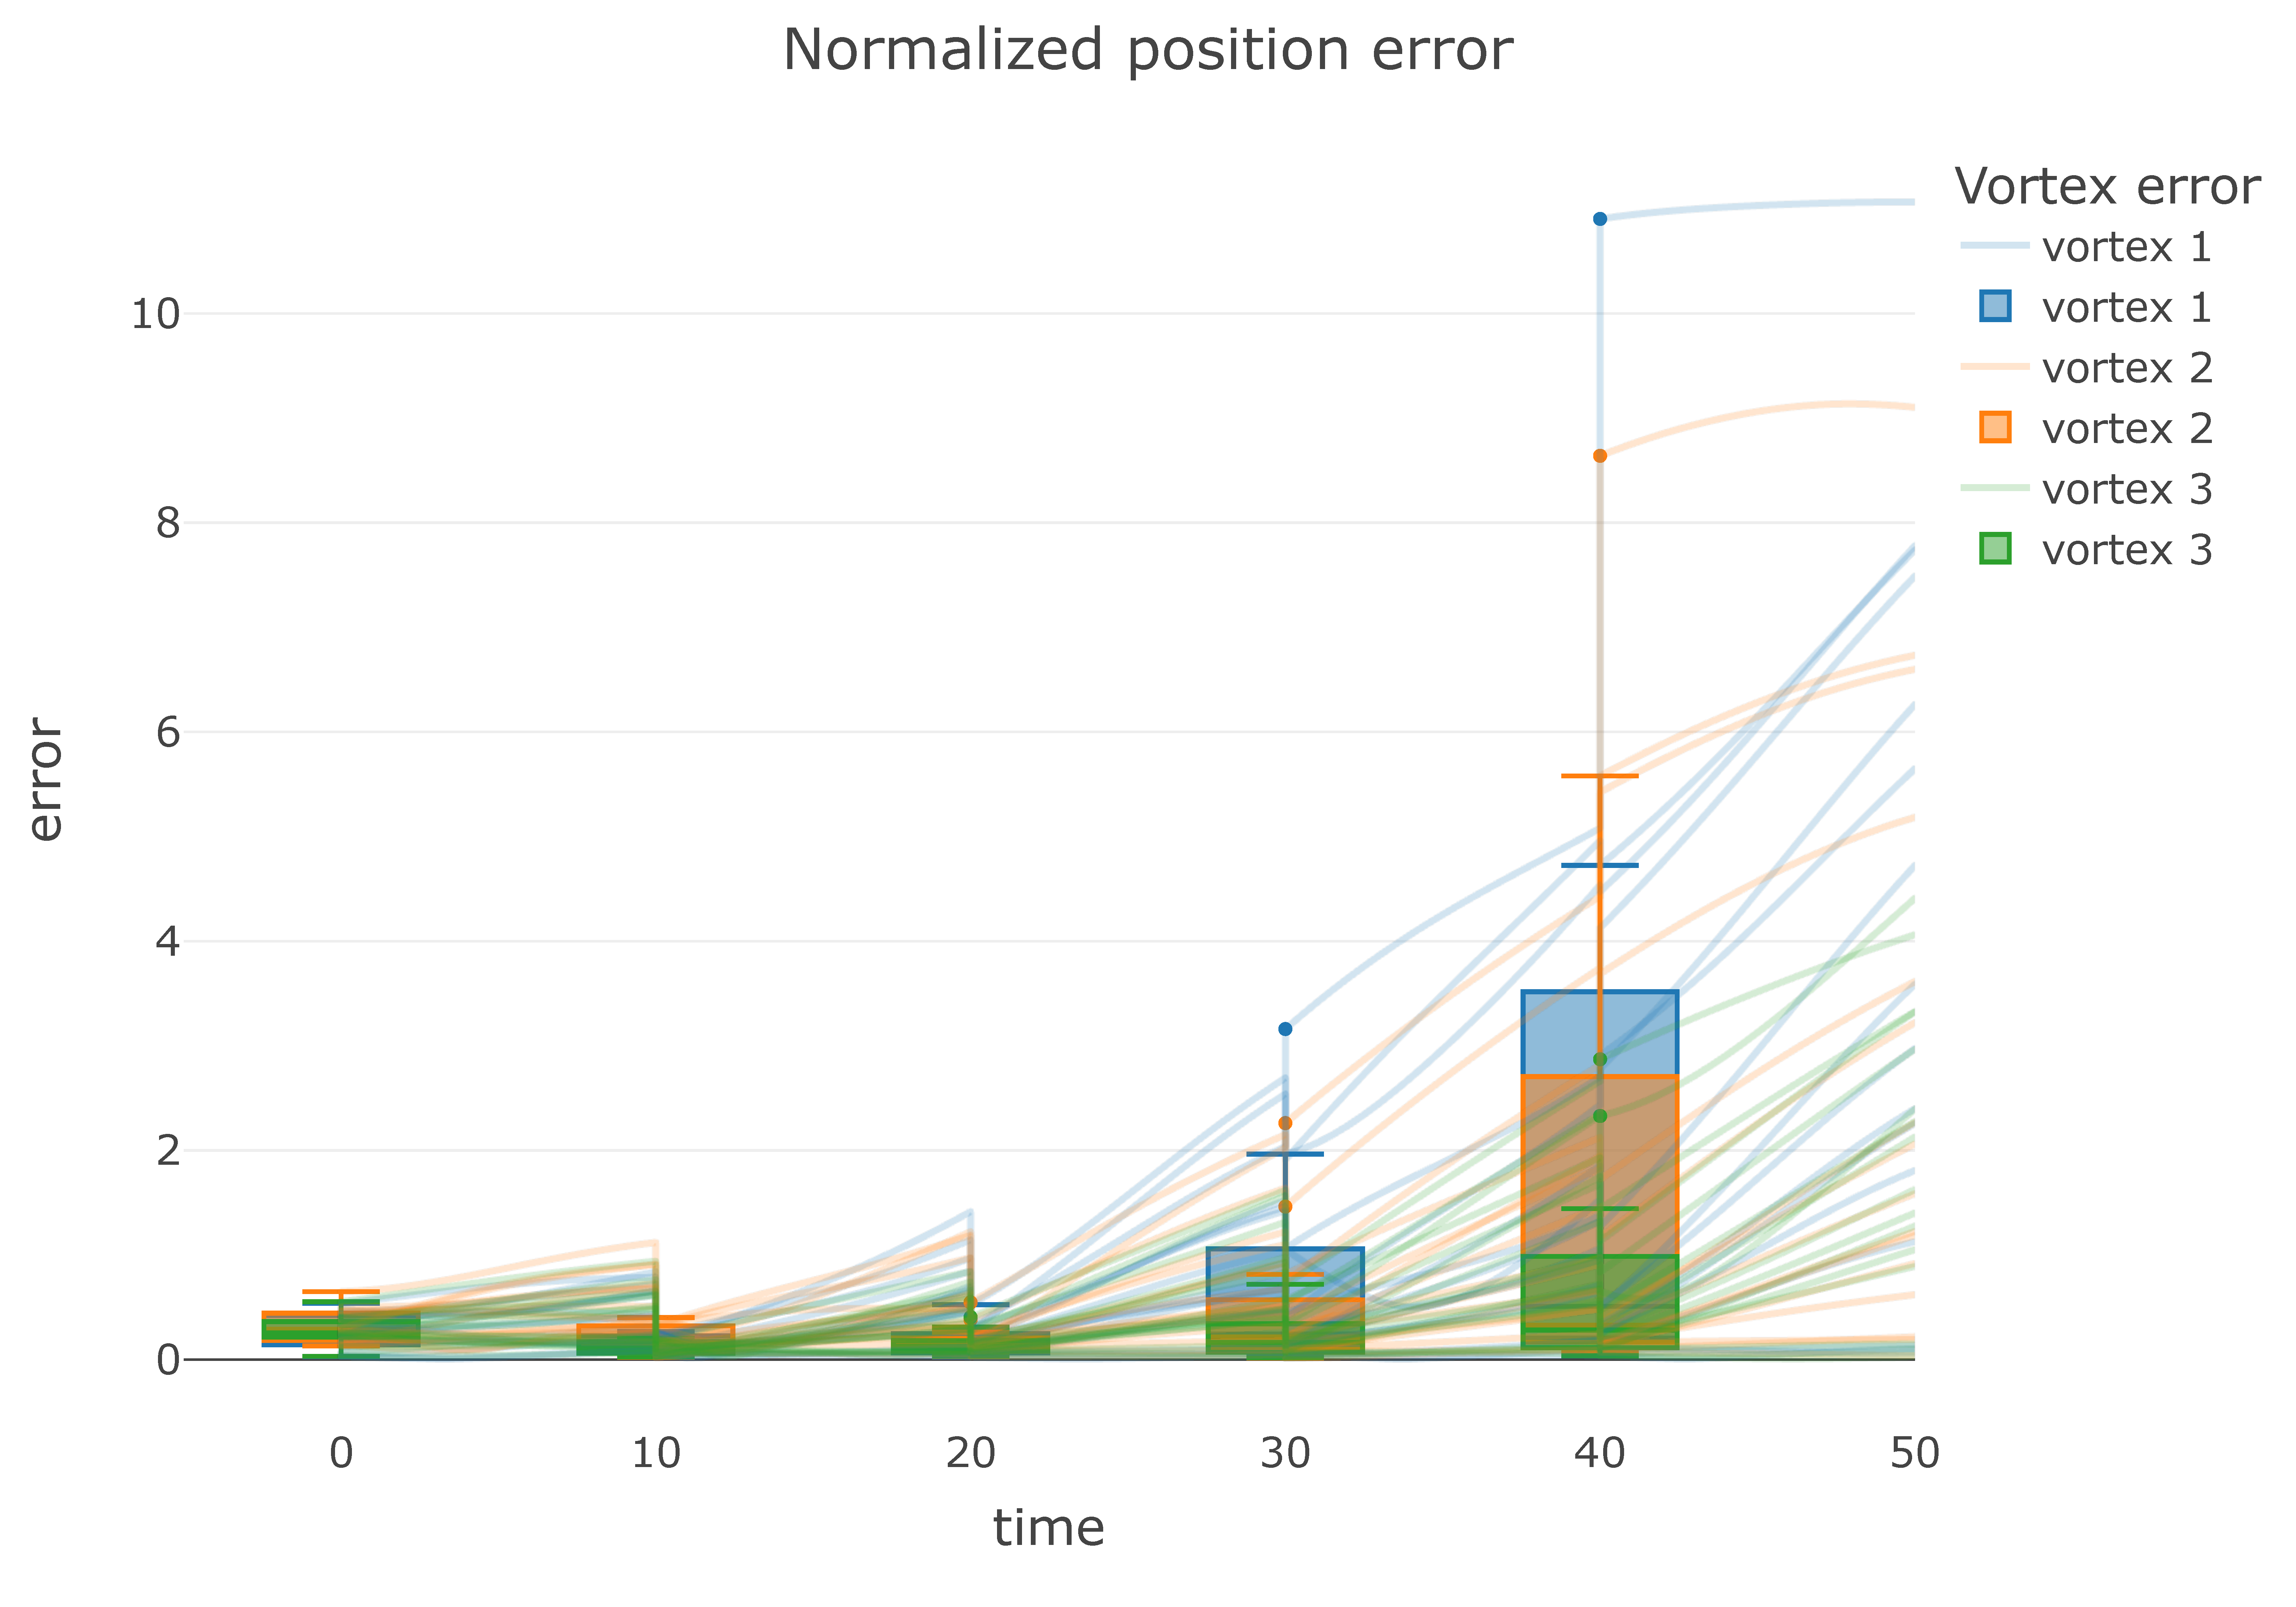
\includegraphics[width=\textwidth]{../../conference/images/part_enkf_error.pdf}
            \end{figure}

            \begin{itemize}
                \item \textbf{pas un cas pratique} pour appliquer le filtre Part-EnKF
            \end{itemize}
        \end{column}
    \end{columns}
\end{frame}

\begin{frame}{Correction de la position}
    \vspace{-0.5cm}
    \begin{columns}[c]
        \begin{column}{0.45\textwidth}
            \begin{figure}
                \centering
                \caption*{\tiny Alignement du champ du membre un lors de la première étape d'assimilation.}
                \includegraphics<1>[width=\textwidth]{../../conference/images/align_member/align_member_prior.pdf}
                \includegraphics<2>[width=\textwidth]{../../conference/images/align_member/align_member_prior_field.pdf}
                \includegraphics<3->[width=\textwidth]{../../conference/images/align_member/align_member_final.pdf}
            \end{figure}
        \end{column}
        \begin{column}{0.55\textwidth}
            \begin{figure}[c]
                \centering
                \caption*{\tiny Correction du champ de vorticité lors de la première étape d'assimilation.}
                \begin{subfigure}{0.49\textwidth}
                    \centering
                    \includegraphics<1-2>[width=\textwidth]{../../conference/images/vorticity_prior.pdf}
                    \only<1-2>{\caption*{\tiny Avant alignement}}
                    \includegraphics<3>[width=\textwidth]{../../conference/images/vorticity_align.pdf}
                    \only<3>{\caption*{\tiny Après alignement}}
                \end{subfigure}
                \begin{subfigure}{0.49\textwidth}
                    \centering
                    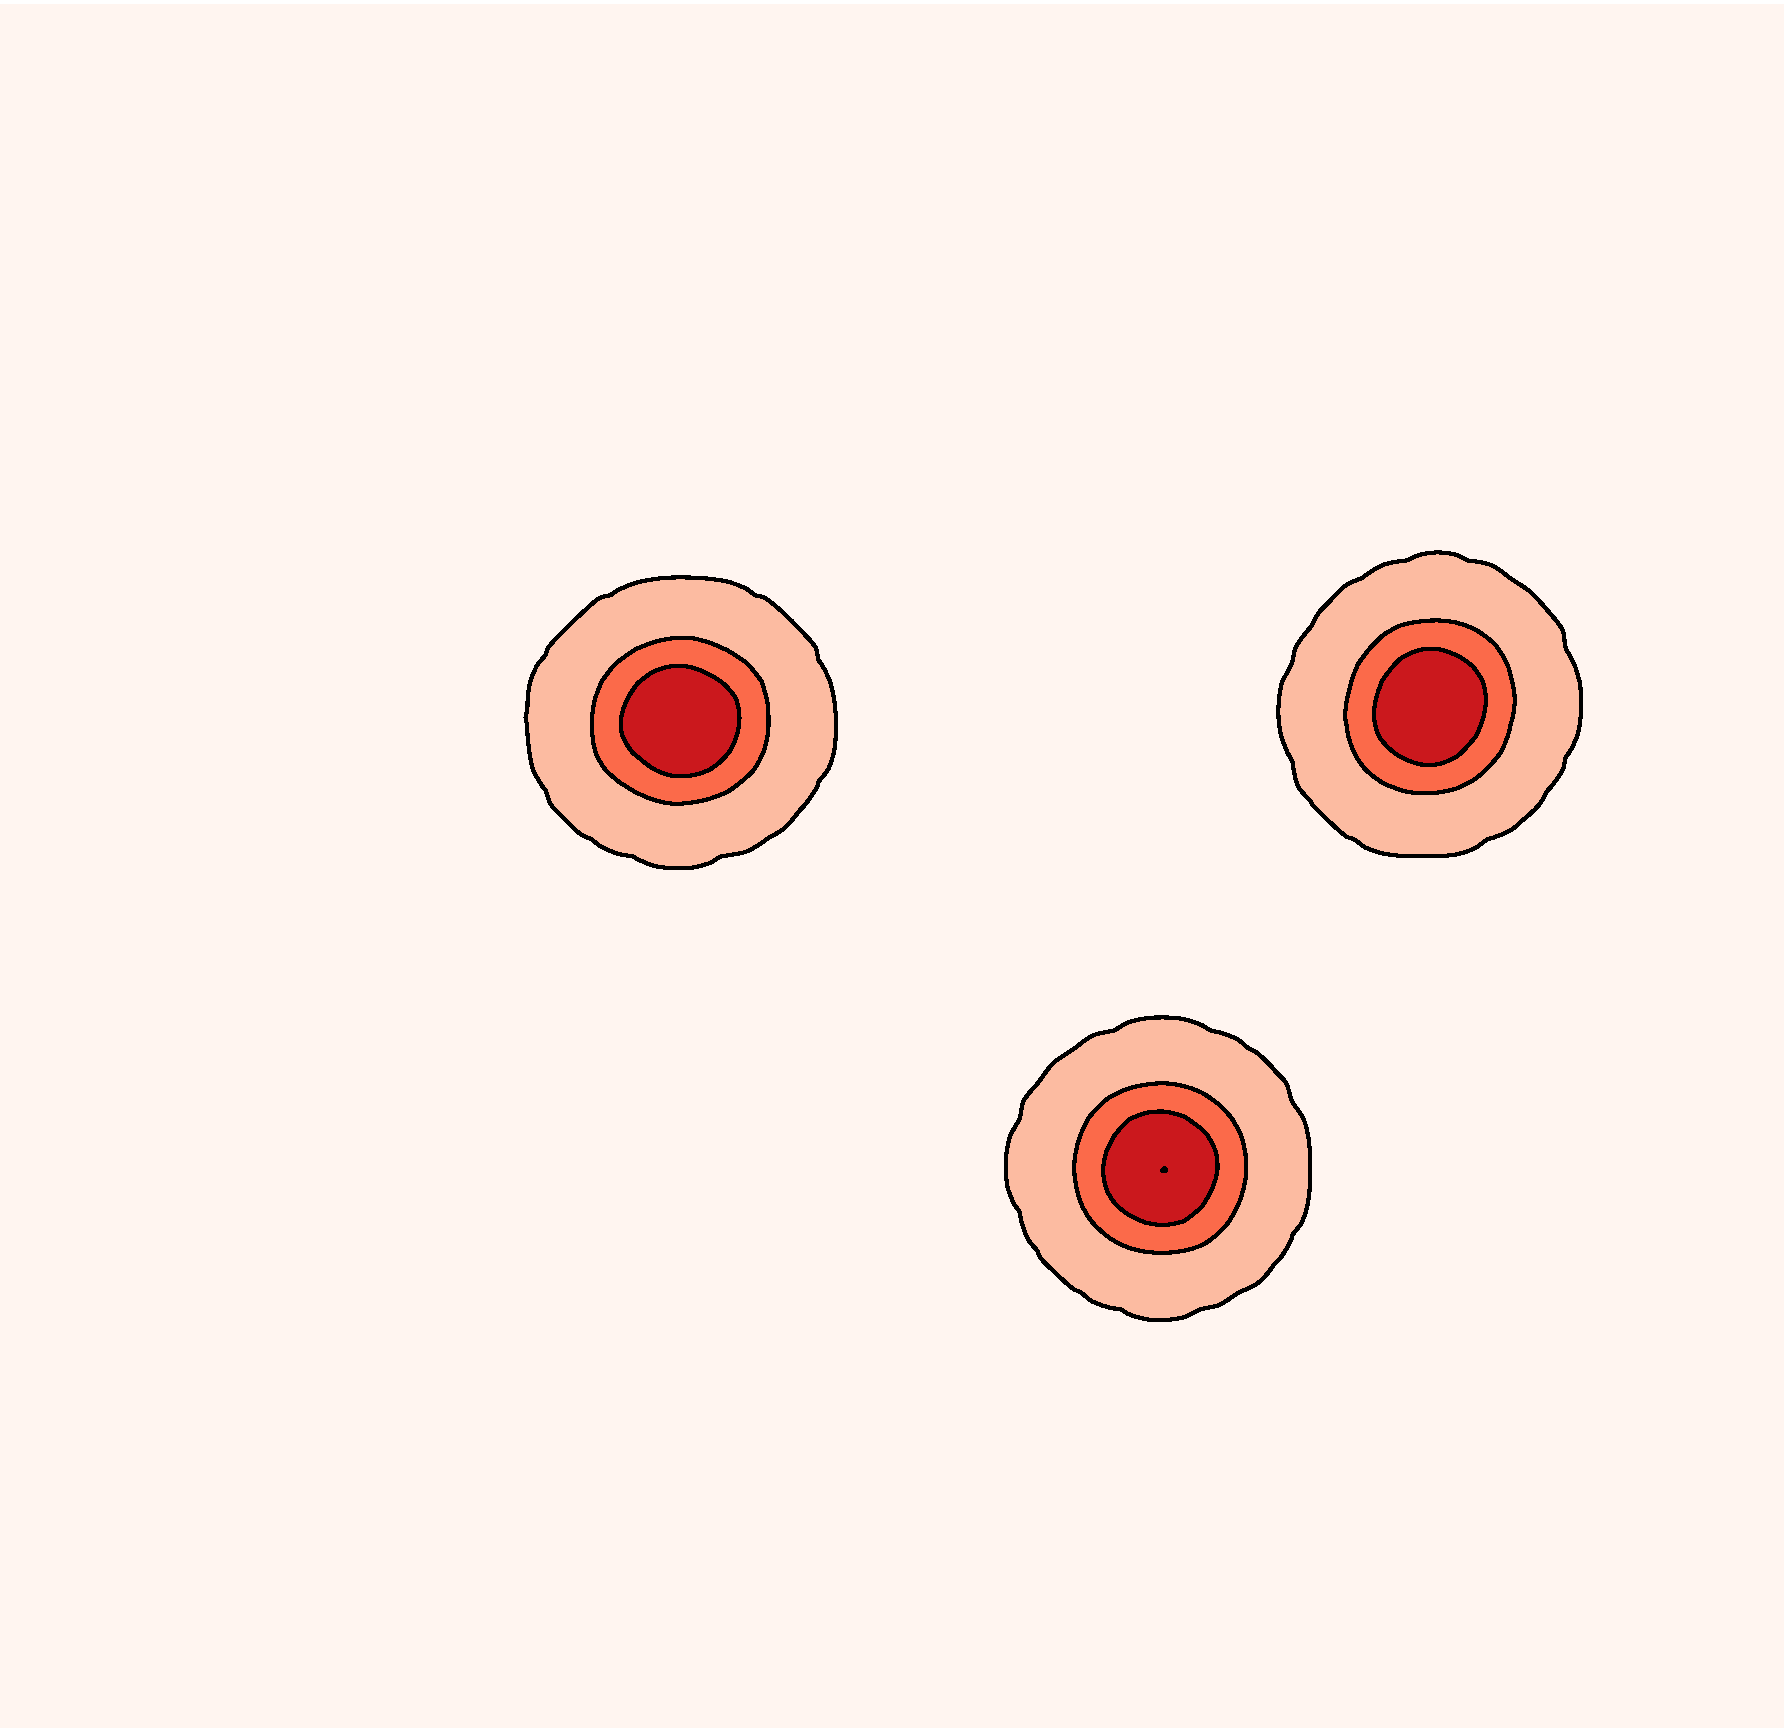
\includegraphics[width=\textwidth]{../../conference/images/vorticity_ref.pdf}
                    \caption*{\tiny Référence}
                \end{subfigure}
            \end{figure}
        \end{column}
    \end{columns}
    \vspace{-0.25cm}
\end{frame}

\begin{frame}{Correction de la position}
    \vspace{-0.5cm}
    \begin{columns}
        \begin{column}{0.5\textwidth}
            \begin{figure}
                \centering
                \animategraphics[loop, autoplay, width=\textwidth]{10}{../../conference/images/vortex_centers_align/vortex_centers_}{0}{36}
                % \caption*{Vortex center trajectories}
            \end{figure}
        \end{column}
        \begin{column}{0.5\textwidth}
            \begin{figure}
                \centering
                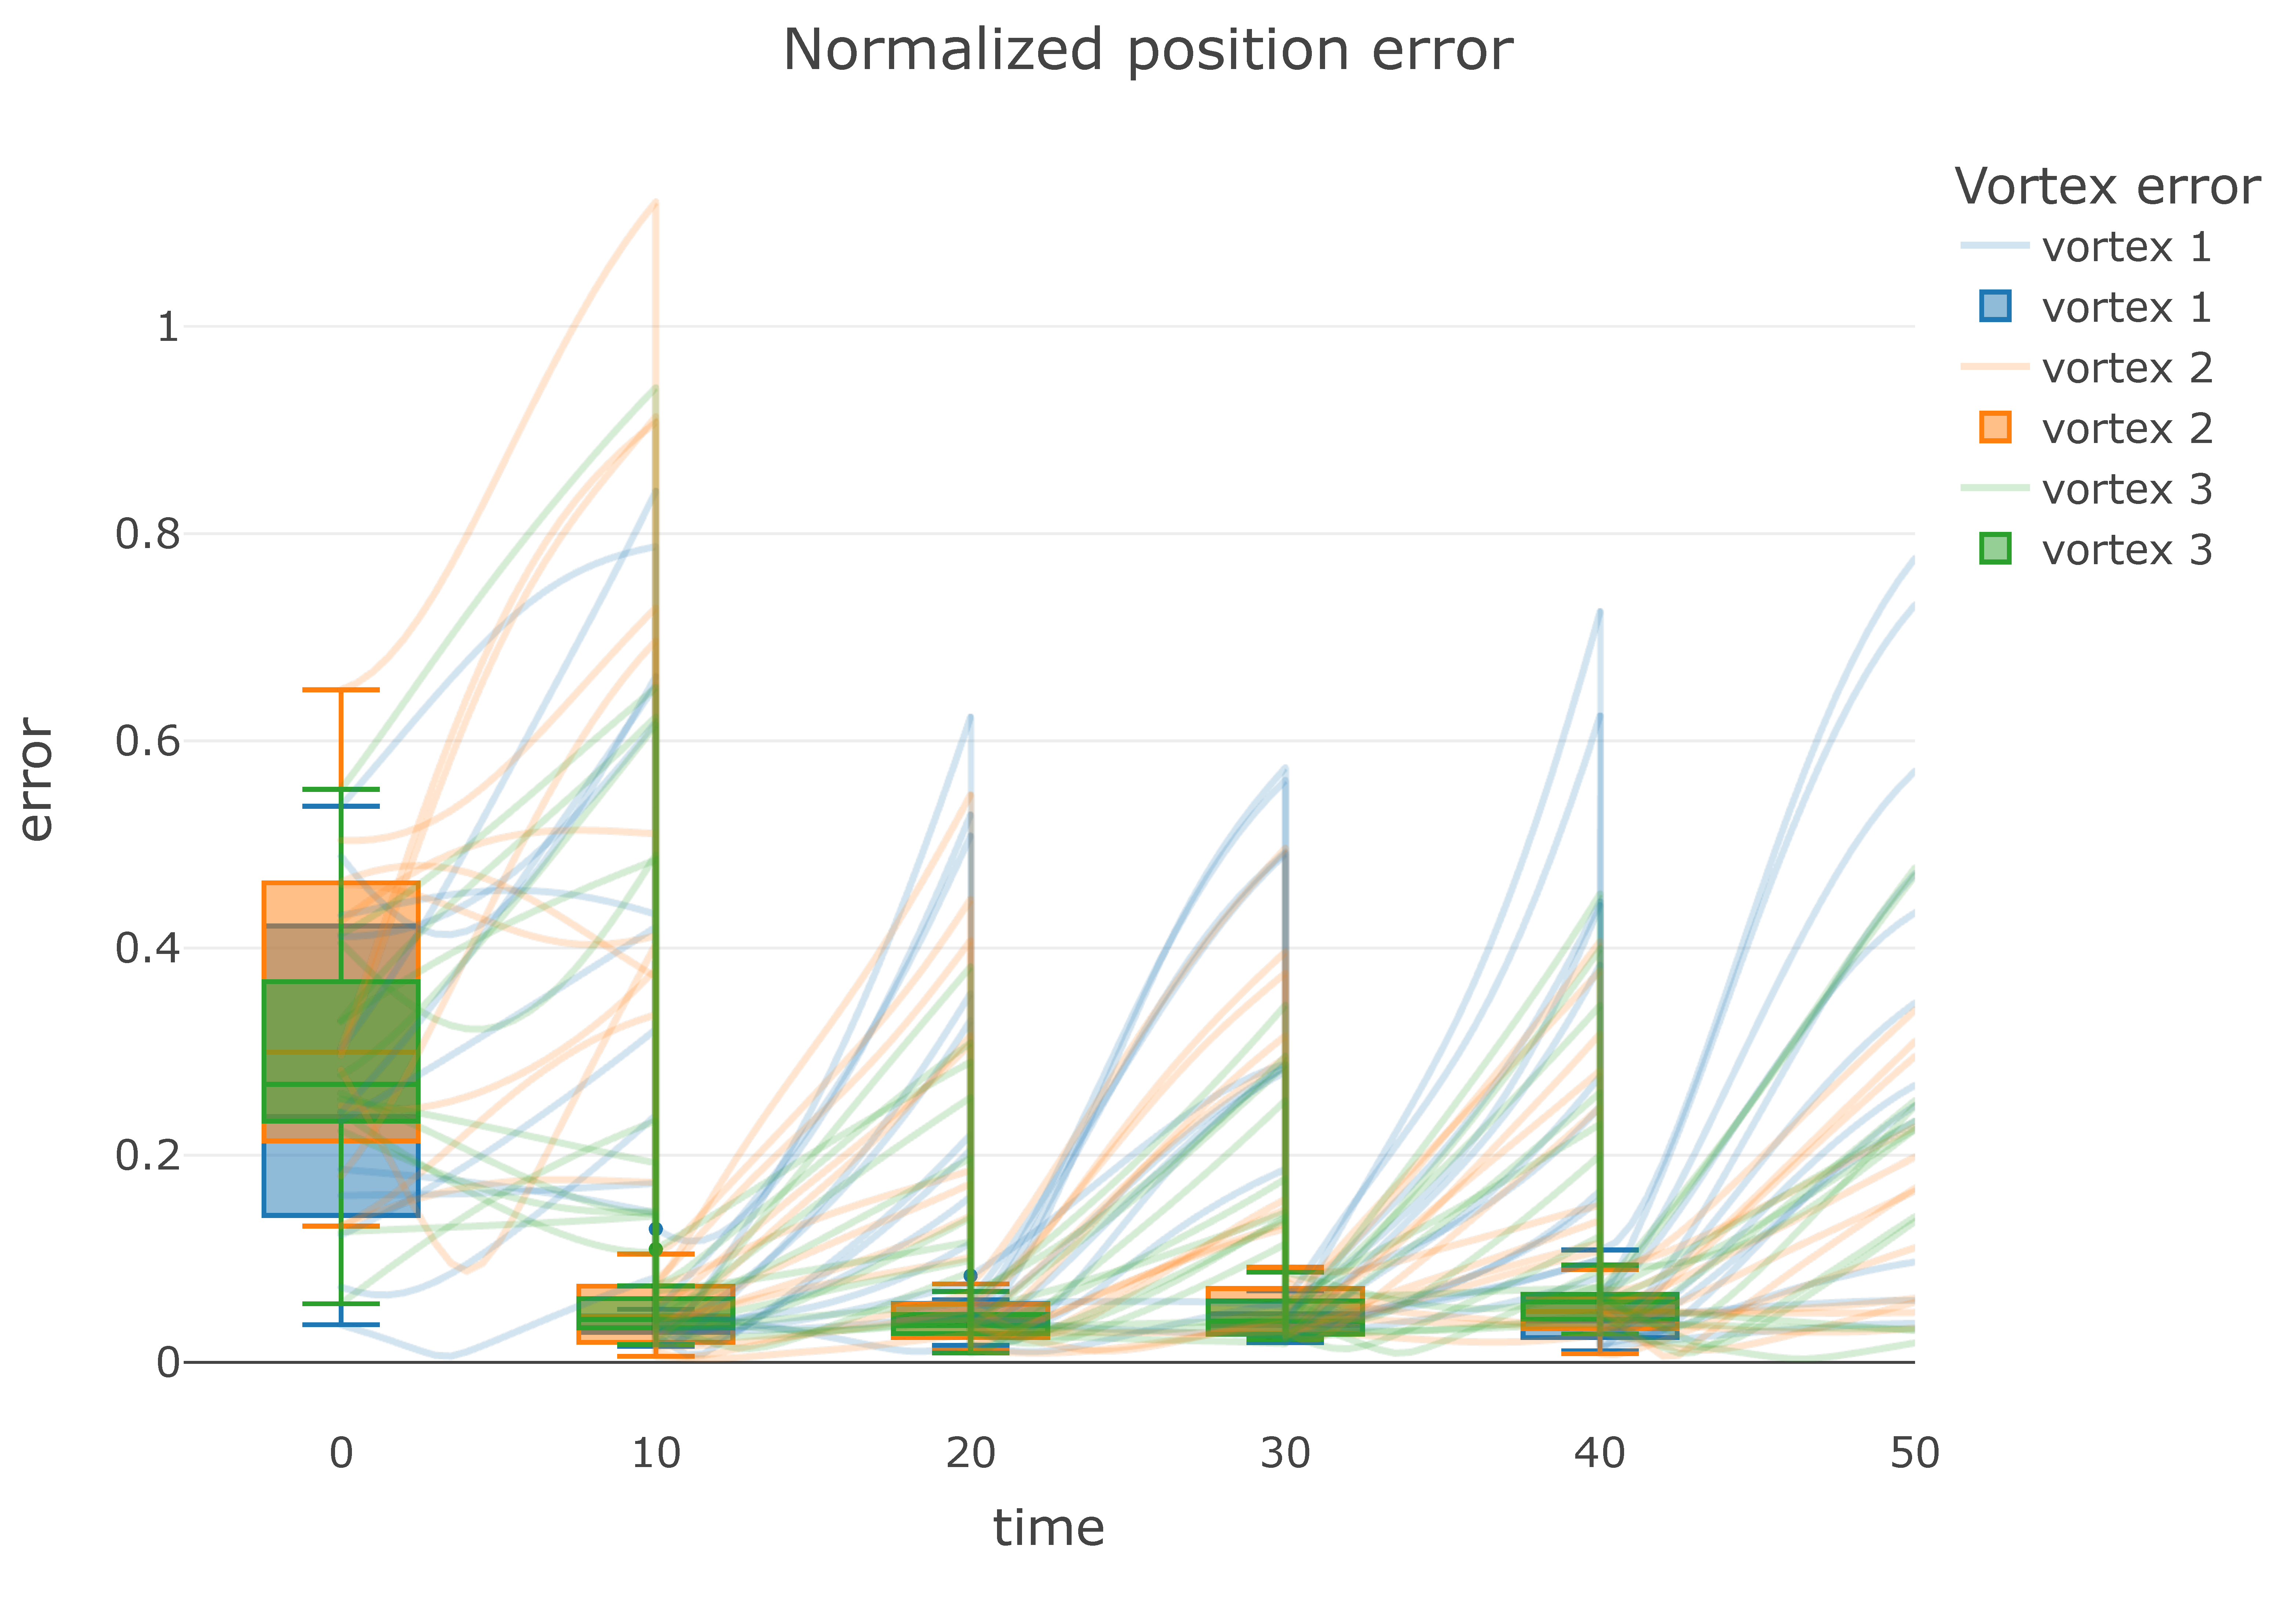
\includegraphics[width=\textwidth]{../../conference/images/align_error.pdf}
                % \caption*{Vortex position error}
            \end{figure}
            \begin{itemize}
                \item Correction de l'erreur de position à chaque assimilation
                \item Mais variabilité à cause de l'incertitude sur les intensités
            \end{itemize}
        \end{column}
    \end{columns}
\end{frame}

\begin{frame}{Correction de la position et de l'intensité}
    \vspace{-0.5cm}
    \begin{columns}
        \begin{column}{0.5\textwidth}
            \begin{figure}
                \centering
                \animategraphics[loop, autoplay, width=\textwidth]{10}{../../conference/images/vortex_centers_part_align/vortex_centers_}{0}{36}
                % \caption*{Vortex center trajectories}
            \end{figure}
        \end{column}
        \begin{column}{0.5\textwidth}
            \begin{figure}
                \centering
                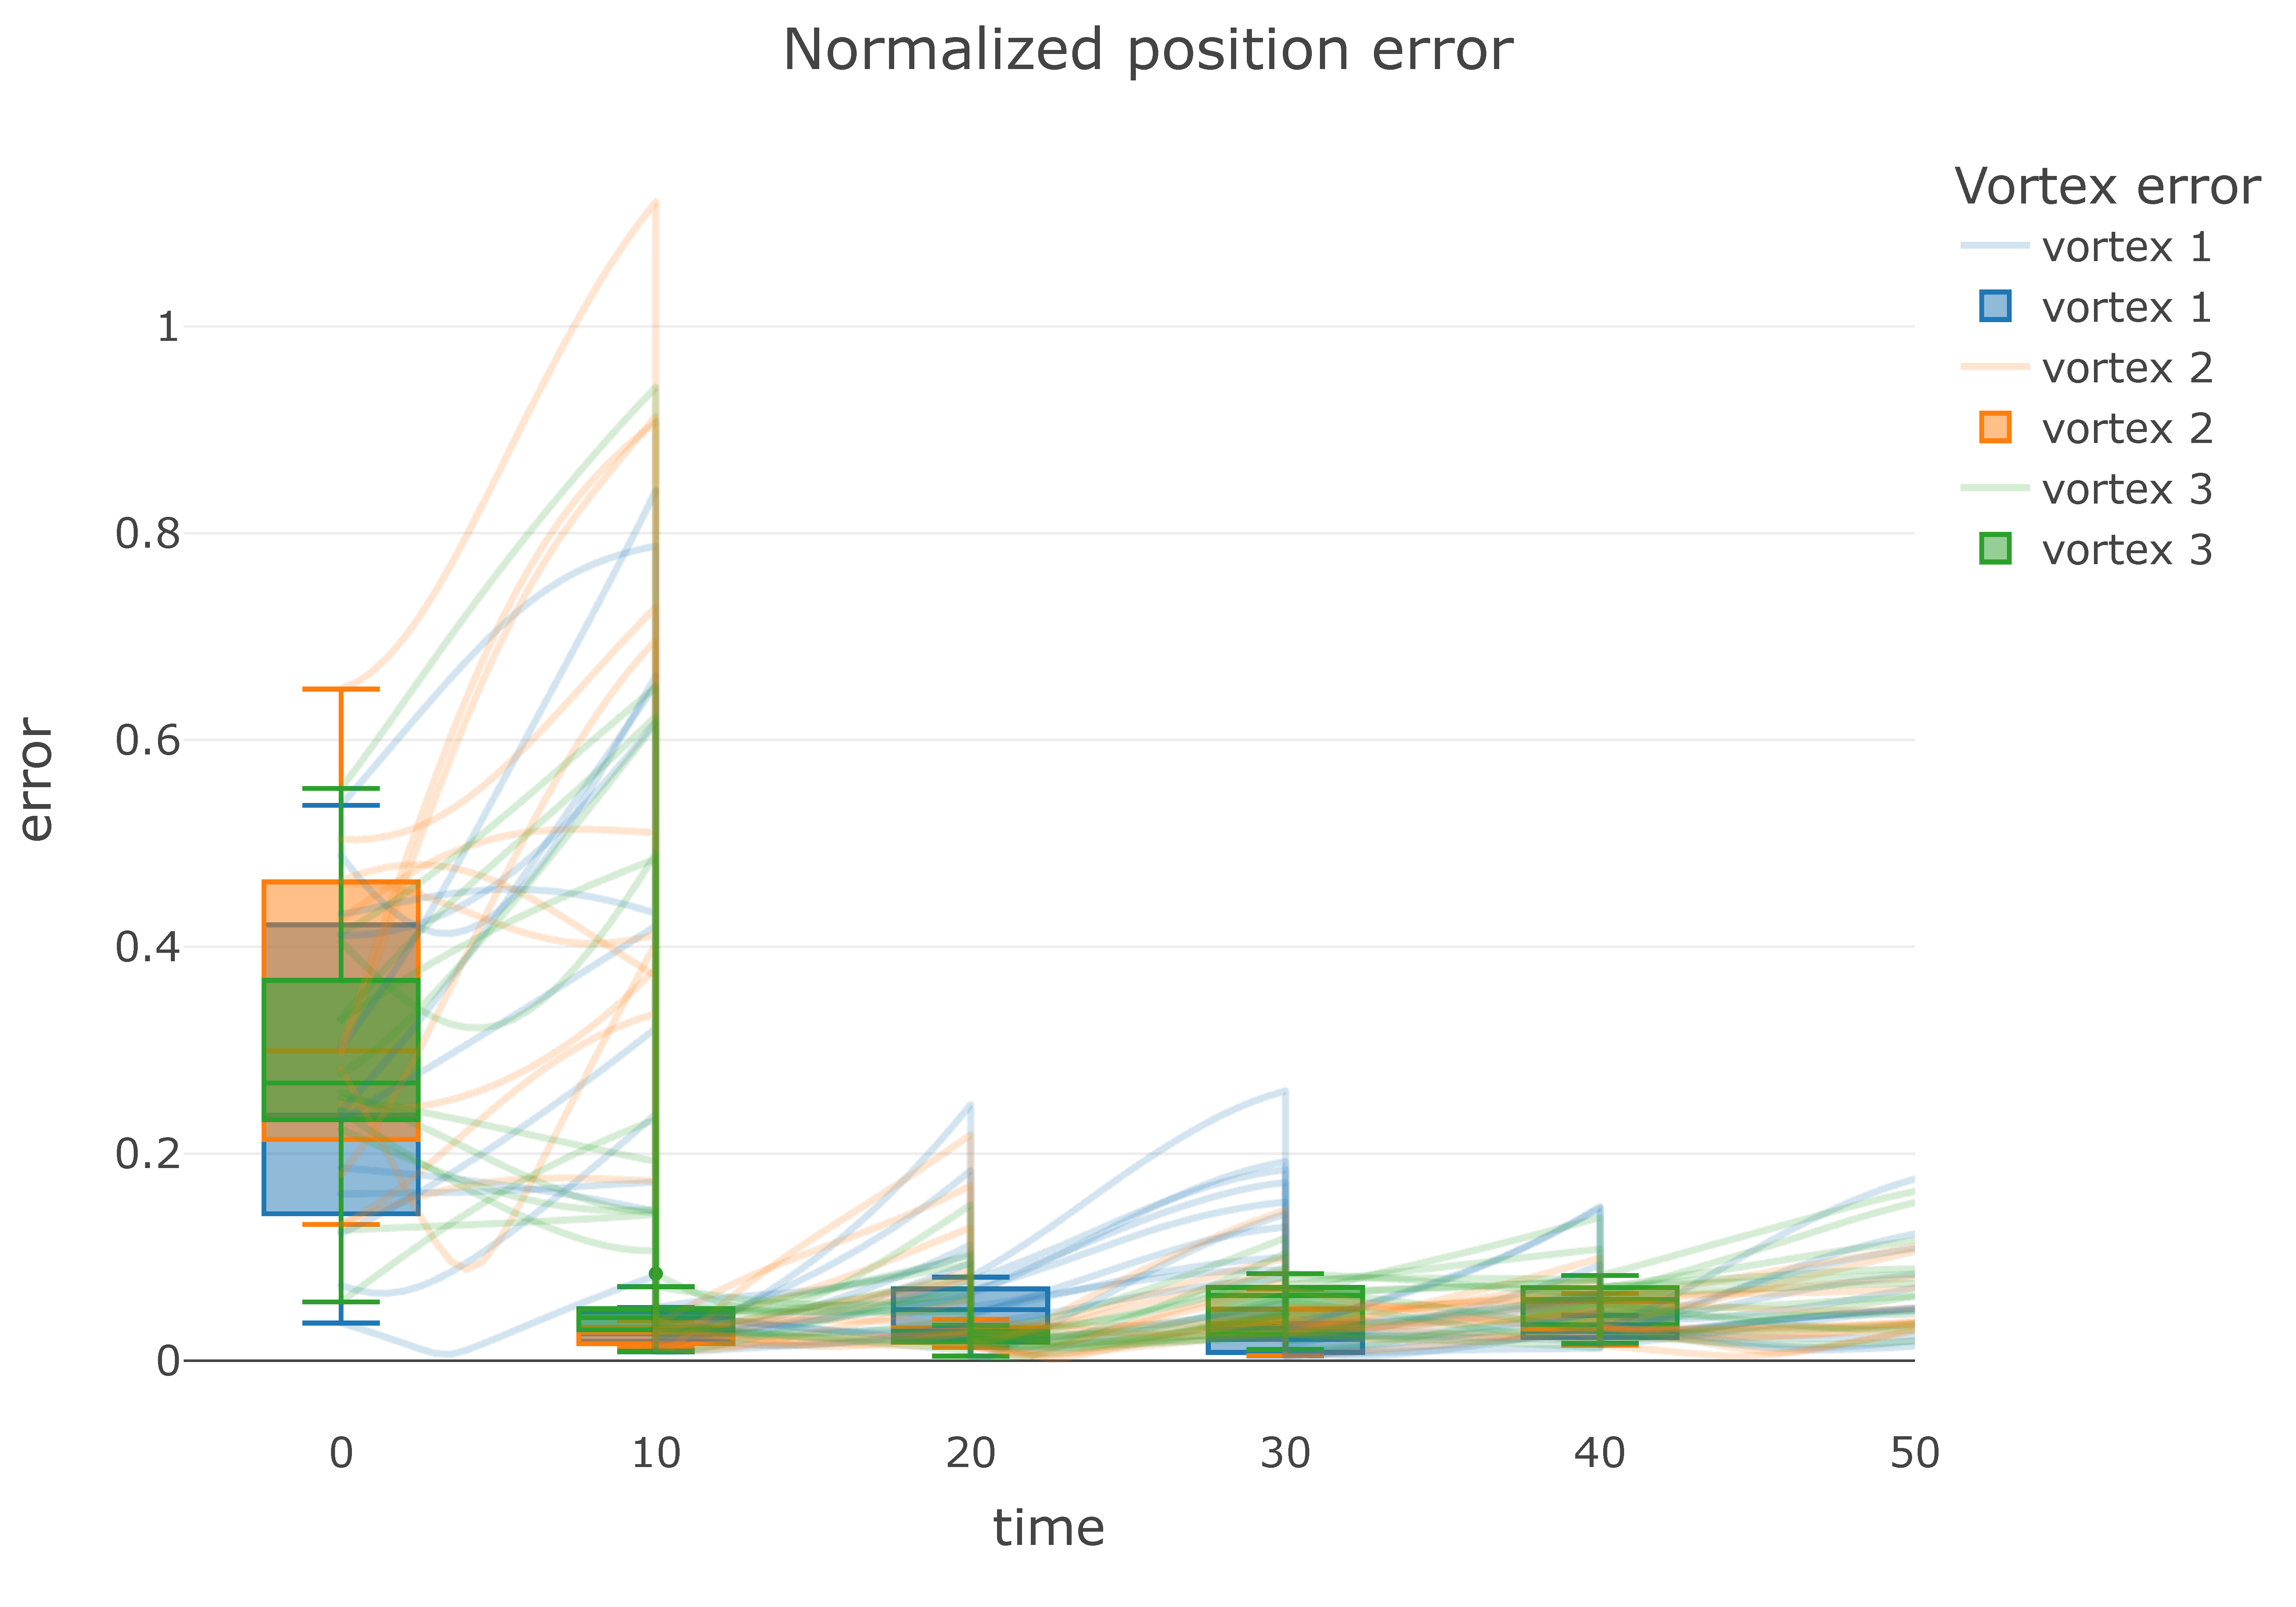
\includegraphics[width=\textwidth]{../../conference/images/align_part_error.pdf}
            \end{figure}

            Correction séquentielle de la \textbf{position} puis de l'\textbf{intensité}
        \end{column}
    \end{columns}
\end{frame}
\section{Conclusion et perspectives}

%18
\begin{frame}{Contributions}
    \begin{columns}[t]
        \begin{column}{0.33\textwidth}
            \begin{block}{Remesh-EnKF}
                Génère une nouvelle configuration de particules
                $\textcolor{ceared}{u^a_i} = \sum_{p \in \textcolor{ceared}{\mathcal G}} \textcolor{ceared}{\Gamma^a_p} \phi_h(x - \textcolor{ceared}{x_p^a})$ \\
                \begin{figure}[b]
                    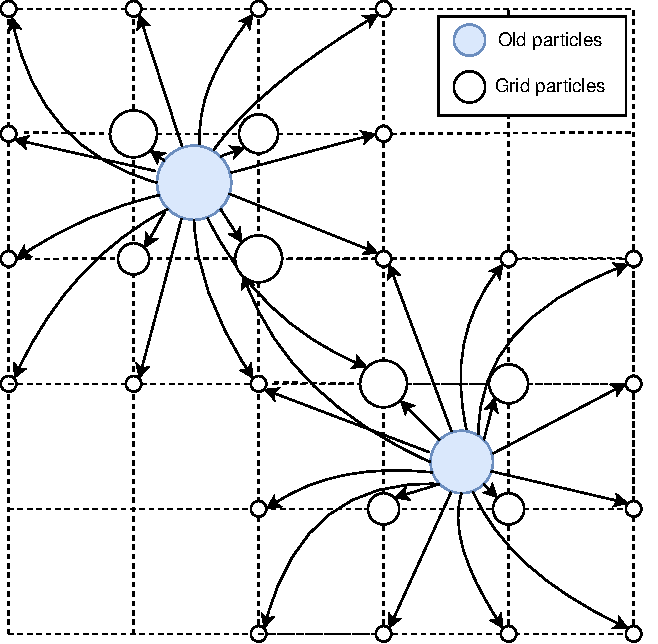
\includegraphics[width=0.8\textwidth]{../../conference/images/redistribution.pdf}
                \end{figure}
            \end{block}
        \end{column}
        \begin{column}{0.33\textwidth}
            \begin{block}{Part-EnKF}
                Correction des intensités
                $\textcolor{ceared}{u^a_i} = \sum_{p \in \mathcal P_i} \textcolor{ceared}{\Gamma^a_p} \phi_h(x - x_p^f)$
                \vfill
                \begin{figure}
                    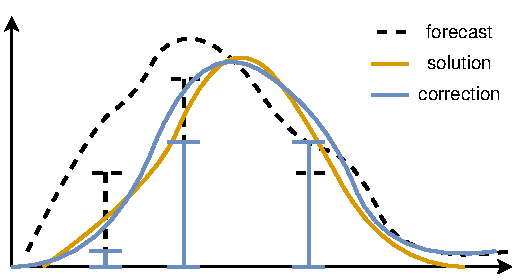
\includegraphics[width=\textwidth]{../../conference/images/correction_final.pdf}
                \end{figure}
            \end{block}
        \end{column}
        \begin{column}{0.33\textwidth}
            \begin{block}{Align-Filter}
                Correction des positions
                $\textcolor{ceared}{u^a_i} = \sum_{p \in \mathcal P_i} \Gamma^f_p \phi_h(x - \textcolor{ceared}{x_p^a})$
                \begin{figure}[b]
                    \centering
                    \includegraphics[width=0.8\textwidth]{../../conference/images/align_member_1.pdf}
                \end{figure}
            \end{block}
        \end{column}
    \end{columns}
\end{frame}

\begin{frame}{Perspectives - MPM / DEM}
    \vspace{-0.5cm}
    \begin{columns}[t]
        \begin{column}{0.5\textwidth}
            \small
            \begin{block}{MPM}
                \begin{figure}[b]
                    \includegraphics[width =0.5\textwidth]{../../conference/images/rot_drum_part/rot_drum_part-81.png}
                \end{figure}
                \begin{itemize}
                    \item \textcolor{green}{\cmark  Remesh-EnKF}\\
                    \item \textcolor{green}{\cmark  Part-EnKF}\\
                    \item \textcolor{green}{\cmark  Align-Filter}
                \end{itemize}
                Champ scalaire à champ vectoriel
            \end{block}
        \end{column}
        \begin{column}{0.5\textwidth}
            \begin{block}{DEM}
                \begin{figure}
                    \includegraphics[width =0.5\textwidth]{../CSI_2024/image/rot_drum_dem/rot_drum_dem-101.png}
                \end{figure}
                \begin{itemize}
                    \item \textcolor{ceared}{\xmark  Remesh-EnKF}\\
                    \item \textcolor{orange}{\cmark  Part-EnKF}\\
                    \item \textcolor{orange}{\cmark  Align-Filter}
                \end{itemize}
            \end{block}
        \end{column}
    \end{columns}
\end{frame}

\begin{frame}{Perspectives - DEM}
    \begin{itemize}
        \item     On choisit d'écrire $A(x)$ comme la solution de \\
              \begin{equation*}
                  \begin{cases}
                      x'(\tau = 0) = x,                                           \\
                      \frac{d x'}{d \tau} = w_i (x'), \quad A_i(x) = x'(\tau = 1) \\
                  \end{cases}
              \end{equation*}
              Intégration avec un schéma prédicteur-correcteur
        \item  Résolution de l'équation de la dynamique $\Rightarrow$ équation du second ordre \\
              \begin{equation*}
                  \begin{cases}
                      x'(\tau = 0) = x,                                                                                               \\
                      \frac{d^2 x'}{dt^2} = \sum_{i=1}^{N_p}f^c_{i}(x') + \textcolor{ceared}{f_{DA}(x')}, \quad A_i(x) = x'(\tau = 1) \\
                  \end{cases}
              \end{equation*}
    \end{itemize}


\end{frame}


% Présenter le cas de MPM
% Présenter le cas DEM
\closingframe

\begin{frame}[allowframebreaks, noframenumbering]
    \frametitle{References}
    \printbibliography % Print the bibliography
\end{frame}

% \section*{Addendum}
% \begin{frame}{EnKF update}
%   \emph{Be successful with your presentation!}
% \end{frame}

\end{document}